\chapter{Temuan dan Pembahasan}
Pada bab ini disajikan berbagai temuan dan pembahasan secara komprehensif terhadap tahap-tahap pelaksanaan eksperimen dan pengujian yang berhasil dilakukan pada setiap skenario yang telah dirancang.

\section{\textit{Data Cleansing}}
Set data FER-2013 didistribusikan resmi dalam sebuah \textit{file} teks CSV\footnote{CSV atau \textit{Comma-Separated Value}, merupakan format \textit{file} teks khusus berbentuk tabel di mana setiap nilai dipisahkan menggunakan tanda koma.} berukuran 301,1MB. Sementara itu, pemuatan \textit{file} menggunakan pustaka \textit{pandas} hanya memerlukan memori sebesar 291,2MB. \textit{File} tersebut terdiri dari 35.887 baris dan 3 kolom, yaitu \textit{emotion}, \textit{pixels} dan \textit{Usage}. Setiap kolom berturut-turut memuat 7 label emosi dalam rentang nilai integer 0--6 (0: \textit{angry}, 1: \textit{disgust}, 2: \textit{fear}, 3: \textit{happy}, 4: \textit{sad}, 5: \textit{surprise} dan 6: \textit{neutral}), 2.304 piksel gambar dalam rentang nilai 0--255 dan 3 jenis penggunaan yang unik (\textit{Training}: set data \textit{training}, \textit{PrivateTest}: set data \textit{validation} dan \textit{PublicTest}: set data \textit{testing}). Adapun distribusi data telah dijelaskan pada bab yang sebelumnya.

Berdasarkan pengecekan secara hati-hati dan menyeluruh, setiap entri data adalah unik. Sehingga dapat dipastikan bahwa tidak ada irisan entri data yang sama untuk penggunaan yang berbeda. Meskipun dalam pemeriksaan singkat, ditemukan beberapa gambar yang terlihat sangat mirip. Namun hal ini tidak akan menjadi masalah, sebab tidak ada data gambar yang memiliki piksel-piksel yang tepat sama.

\textit{Data cleansing} dimulai dengan pemeriksaan data rusak, tidak relevan atau tidak lengkap. Pemeriksaan khusus data gambar dilakukan secara manual satu per satu supaya menyeluruh dan akurat. Alhasil disimpulkan bahwa setiap entri data adalah lengkap. Sayangnya, sejumlah data gambar sebanyak kurang lebih 85 buah ditemukan rusak, yaitu data gambar ke-59, 2059, 2171, 2809, 3262, 3931, 4275, 5082, 5274, 5439, 5722, 5881, 6102, 6458, 6699, 7172, 7496, 7527, 7629, 8030, 8737, 8856, 9026, 9500, 9673, 9679, 10423, 11244, 11286, 11295, 11846, 12289, 12352, 13402, 13697, 13988, 14279, 15144, 15553, 15838, 15894, 17081, 19238, 19632, 20222, 20712, 20817, 21817, 22198, 22314, 22407, 22927, 23596, 23894, 24053, 24441, 24891, 25219, 25603, 25909, 26383, 26860, 26897, 28601, 29447, 29557, 30002, 30705, 30981, 31127, 31825, 32662, 32683, 34334, 35121, 35469, 35632, 35743, 5509, 10023, 11826, 17620, 10219, 14550, dan 15389. Sehingga setiap entri data terkait perlu dihapus. Pada Gambar \ref{fig:contohdatagambarrusak}, ditampilkan beberapa contoh data gambar yang rusak. Yang banyak terlihat di sana adalah gambar sudah tidak dapat diakses kembali dari alamat web semula. Namun, yang membingungkan adalah semua itu masih merupakan \textit{file} gambar, yang mana seolah-olah gambar-gambar tersebut berupa hasil tangkapan layar (\textit{screenshot}).
\begin{figure}[t]
    \centering
    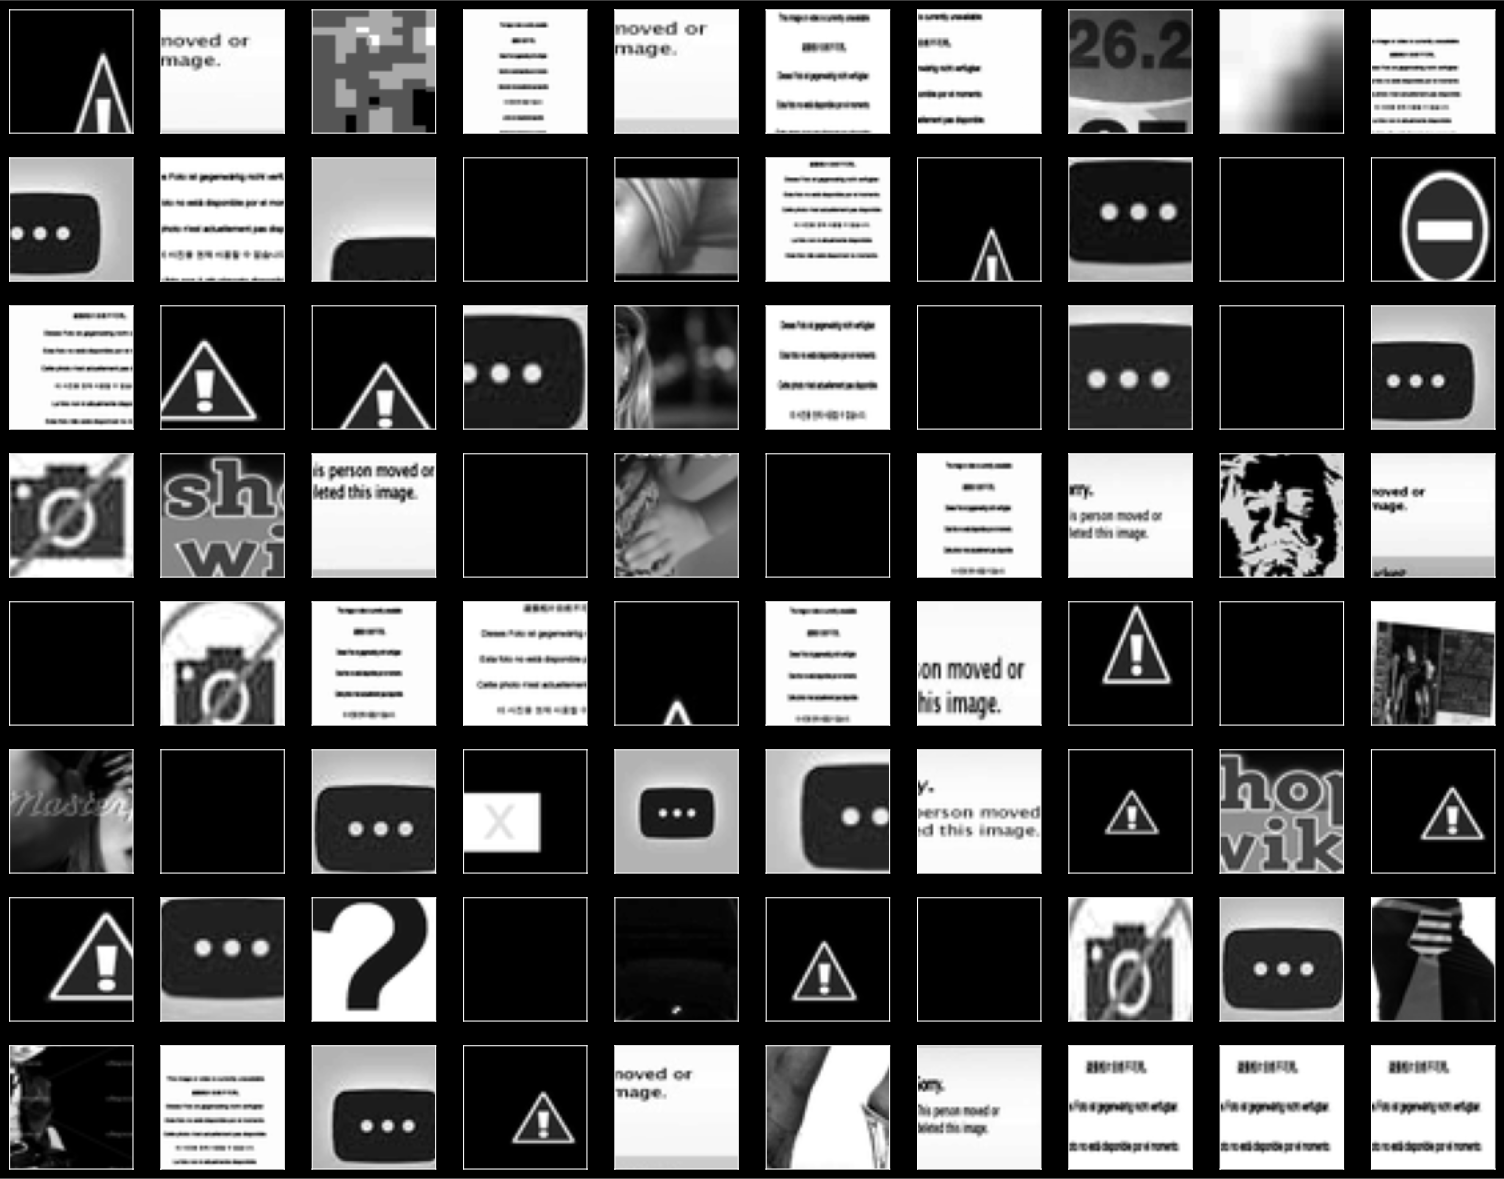
\includegraphics[width=14cm]{gambar/fer2013_data_rusak.png}
    \caption{Beberapa Contoh Data Gambar Rusak pada FER-2013}
    \label{fig:contohdatagambarrusak}
\end{figure}

\section{Praproses Data}
Pada skenario pertama, praproses data diawali dengan memperbesar (\textit{upscaling}) dimensi seluruh data gambar dari 48 $\times$ 48 piksel menjadi 64 $\times$ 64 piksel menggunakan \textit{opencv-python} dalam rangka penyesuaian ukuran set data gambar dengan dimensi lapisan input arsitektur model \acrshort{cnn} \textit{baseline}. %Beberapa contoh hasil proses ini dapat dilihat pada Gambar \ref{fig:contohupscaling}, di mana menghasilkan gambar yang tampak lebih halus meskipun tanpa interpolasi.
Selanjutnya, penulis mencoba menemukan teknik \textit{image enchancement} yang paling cocok untuk meningkatkan kualitas atau keterbacaan tiap-tiap gambar. Teknik-teknik yang akan penulis uji coba hanya berkisar pada teknik \textit{illumination normalization}. Namun, sebelum menerapkan teknik-teknik tersebut, penulis mengambil beberapa sampel gambar yang memiliki karakteristik yang cukup jauh. Dengan harapan bahwa sejumlah gambar tersebut dapat mewakili setiap variasi karakteristik gambar yang akan dikenakan teknik \textit{enhancement}.
% \begin{figure}[t]
%     \centering
%     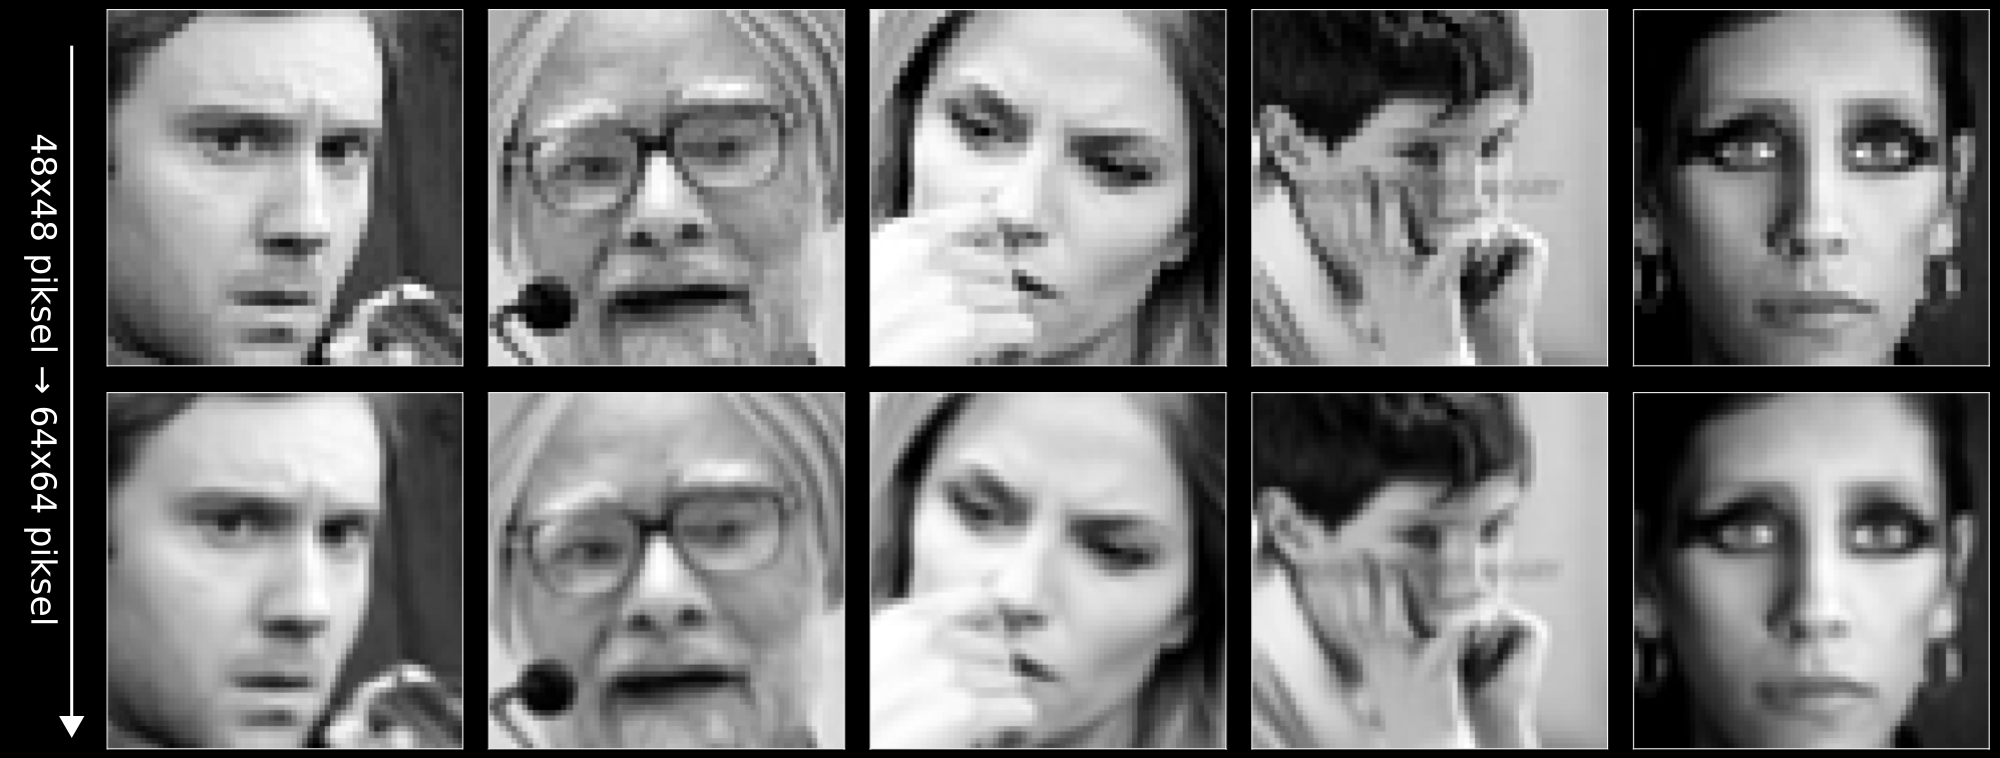
\includegraphics[width=14cm]{gambar/fer2013_contoh_upscaling.png}
%     \caption{Beberapa Contoh Hasil Proses \textit{Upscaling} terhadap FER-2013 dalam Ukuran yang Diseragamkan}
%     \label{fig:contohupscaling}
% \end{figure}

\begin{figure}
    \centering
    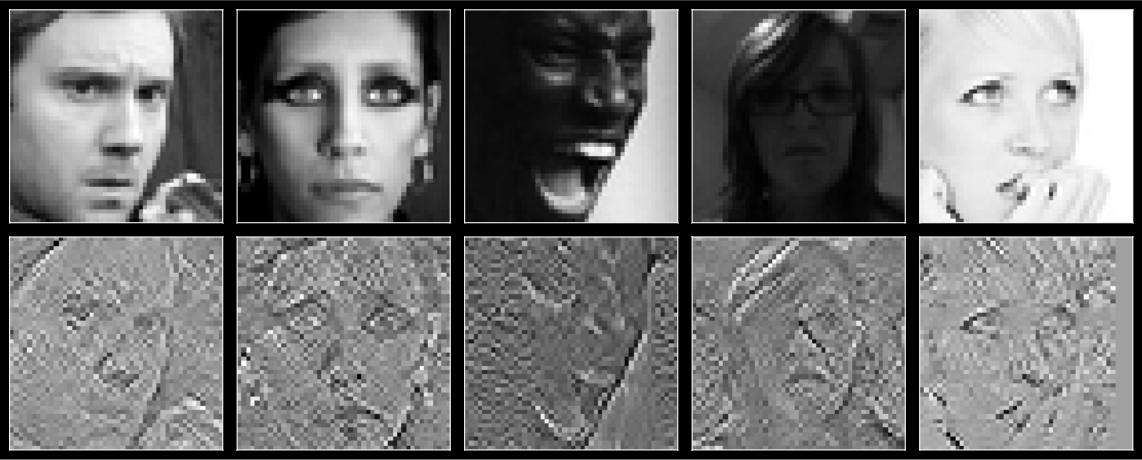
\includegraphics[width=14cm]{gambar/contoh_zca2.png}
    \caption{Beberapa Contoh Hasil Implementasi \acrshort{zca} terhadap FER-2013}
    \label{fig:contohzca2}
\end{figure}
Teknik pertama adalah \textit{image whitening} menggunakan \acrshort{zca} untuk menggantikan proses normalisasi yang disebutkan pada penelitian \textit{baseline}. Kode programnya diambil dari https://github.com/mwv/zca. Sayangnya, sebagaimana yang ditunjukkan pada Gambar \ref{fig:contohzca2}, pengenaan teknik ini ternyata menghilangkan banyak sekali informasi spasial mencakup informasi tekstur (seperti kerutan kulit di dahi dan pipi) dan garis tepi. Penulis menduga hal ini disebabkan oleh kecilnya resolusi gambar serta adanya limitasi dari \textit{grayscale}. Kekurangan ini tentunya sangat bertentangan dengan alasan mengapa penulis mengadopsi filter Gabor pada metode penelitian penulis.

\begin{figure}[t]
    \centering
    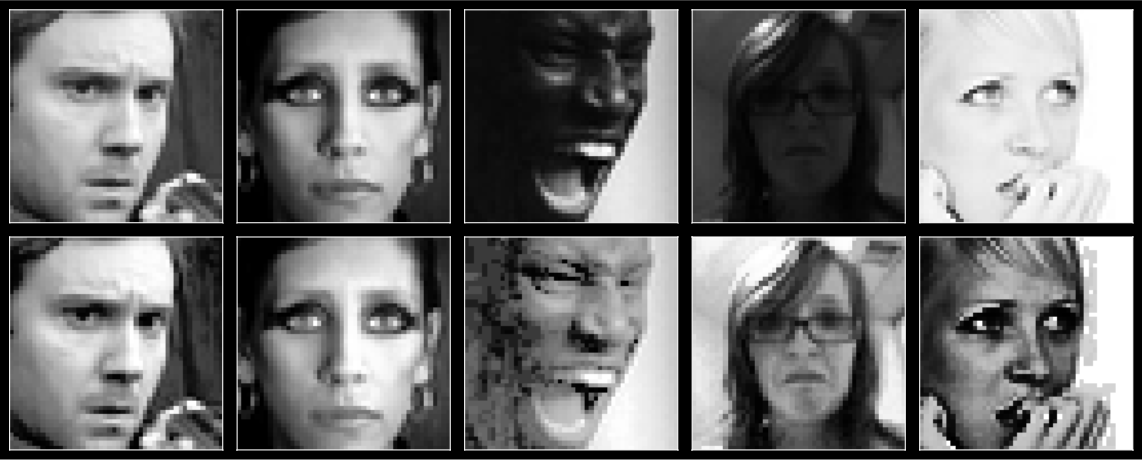
\includegraphics[width=14cm]{gambar/contoh_histogram_equalization.png}
    \caption{Beberapa Contoh Hasil Implementasi \textit{Histogram Equalization} terhadap FER-2013}
    \label{fig:contohhistogramequalization}
\end{figure}
Teknik kedua adalah \textit{histogram equalization} yang cukup populer dan dapat dipercaya terutama untuk meningkatkan kualitas area gambar yang relatif terlalu gelap. Hasilnya dapat dilihat pada Gambar \ref{fig:contohhistogramequalization}. Secara keseluruhan, teknik ini sangat andal dalam meningkatkan kualitas gambar baik yang terlalu gelap maupun terlalu terang. Namun, teknik ini gagal terhadap gambar yang memiliki kontras yang cukup jauh antara objek dan latar. Alhasil, kedua teknik ini tidak akan penulis gunakan pada penelitian ini.

\begin{table}
    \caption[Perbandingan Teknik-Teknik \textit{Facial Landmark Detection}]{Perbandingan Teknik-Teknik Facial Landmark Detection}
    \label{tab:teknikfaciallandmarkdetection}
    \begin{tabular}{|C{3.5cm}|C{2cm}|C{2.1cm}|C{0.8cm}|C{2cm}|C{0.9cm}|}
        \hline
        Pustaka & \textit{Loss} (\%)$^\bigtriangledown$ & Waktu (s)$^\bigtriangledown$ & \textit{n}$^\bigtriangleup$ & \textit{Threshold} & GPU \\
        \hline\hline
        \textit{face\_alignment} (face\_detector=sfd) & \multirow{2}{*}{3,10} & \multirow{2}{*}{2.786} & \multirow{2}{*}{68} & \multirow{6}{*}{0,5} & \multirow{6}{*}{\ding{51}} \\
        \cline{1-4}
        \textit{RetinaFace} (net=mobilenet0.25) & \multirow{2}{*}{42,23} & \multirow{2}{*}{334} & \multirow{4}{*}{5} &  &  \\
        \hhline{*{3}{|-}|~|}
        \textit{RetinaFace} (net=resnet50) & \multirow{2}{*}{7,05} & \multirow{2}{*}{476} &  &  &  \\
        \hline
    \end{tabular}
    \footnotesize
    {\raggedright
    \textit{Loss}---persentase banyak data gambar yang tidak terdeteksi wajah; Waktu---waktu total eksekusi pendeteksian \emph {facial landmark} untuk seluruh data gambar; \textit{n}---banyak \textit{facial landmark} per wajah;\\
    $^\bigtriangleup$Lebih tinggi lebih baik; $^\bigtriangledown$Lebih rendah lebih baik.}
\end{table}
Pada skenario kedua, penulis menambahkan empat langkah ekstra tepat sebelum memasuki tahap \textit{upscaling}. Tahap pertama merupakan pendeteksian area wajah pada setiap gambar dengan batas ambang (\textit{threshold}) sama dengan 0,5. Setiap area wajah yang ditandai dan berhasil melewati \textit{threshold} akan diteruskan ke tahap berikutnya, yaitu pendeteksian atau prediksi \textit{facial landmark}. Kedua tahap ini dapat ditangani baik secara terpisah maupun tergabung oleh berbagai pustaka yang telah tersedia publik. Penulis telah mencoba beberapa di antaranya dan membandingkan metode mana yang paling kredibel untuk diimplementasikan pada set data wajah nonfrontal, FER-2013. Namun, di sini penulis hanya akan membahas hasil dari dua metode terbaik, yaitu \textit{\acrlong{fan}} (\acrshort{fan}) dalam pustaka \textit{face\_alignment} \shortcite{bulat2017far} dan \textit{RetinaFace} \shortcite{deng2019retinaface}.

Sebagaimana yang disimpulkan pada Tabel \ref{tab:teknikfaciallandmarkdetection}, metode \acrshort{fan} unggul dalam kecilnya persentase kehilangan data dan banyaknya \textit{facial landmark} yang mampu diprediksi. Kendati pun waktu eksekusinya sangat lama, hal ini tidak akan menjadi masalah yang penting. Sementara itu, metode \textit{RetinaFace} memiliki waktu eksekusi relatif cukup cepat, namun memiliki persentase kehilangan data yang relatif besar. Terutama metode \textit{RetinaFace} yang menggunakan arsitektur MobileNet0.25, metode \textit{RetinaFace} kurang bisa diandalkan. Akan tetapi, masih perlu validasi tiap-tiap metode dengan mengambil beberapa sampel hasil deteksi \textit{facial landmark}.

\begin{figure}
    \centering
    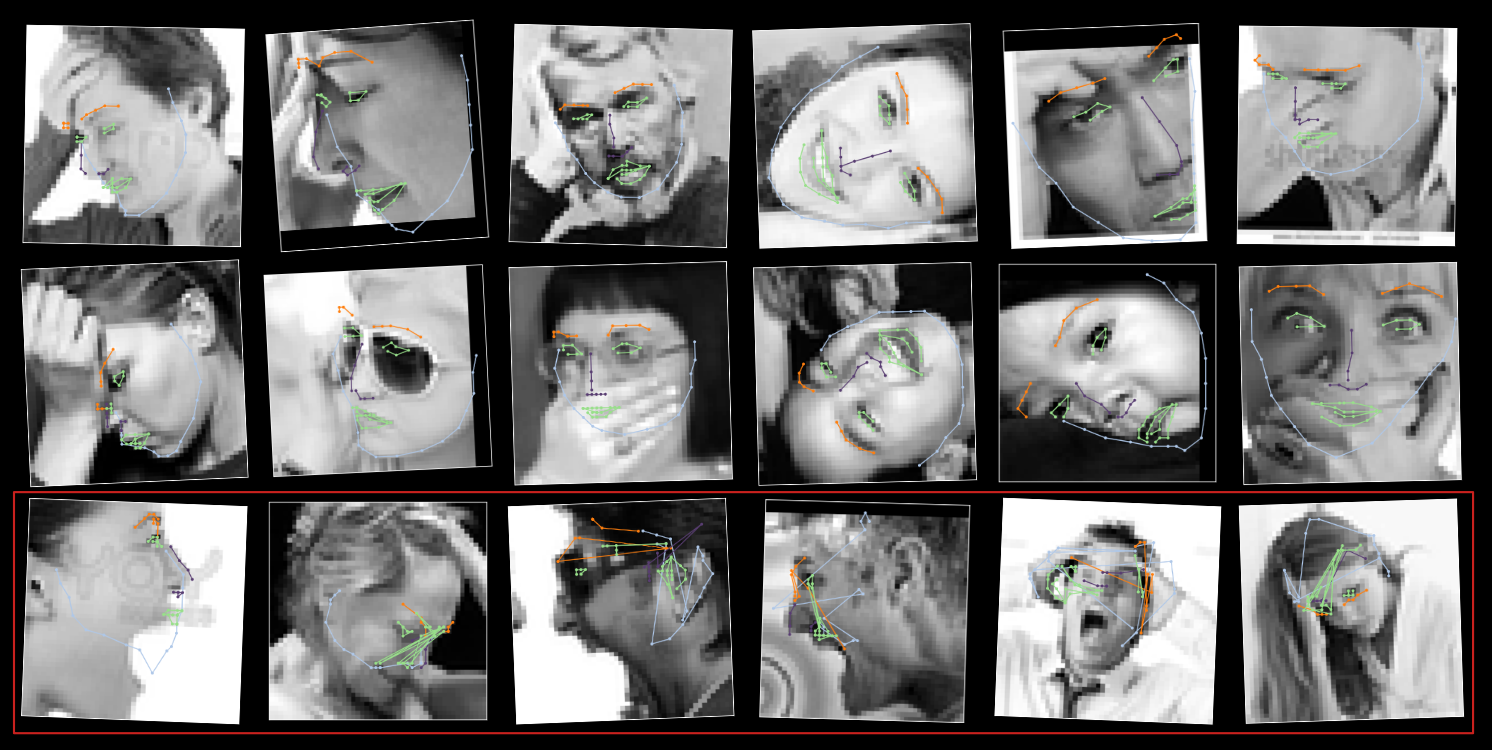
\includegraphics[width=14cm]{gambar/contoh_hasil_facealignment.png}
    \caption{Beberapa Contoh Hasil Deteksi \textit{Facial Landmark} terhadap FER-2013 Menggunakan \acrshort{fan}}
    \label{fig:contohhasilfacealignment}
\end{figure}
\begin{figure}
    \centering
    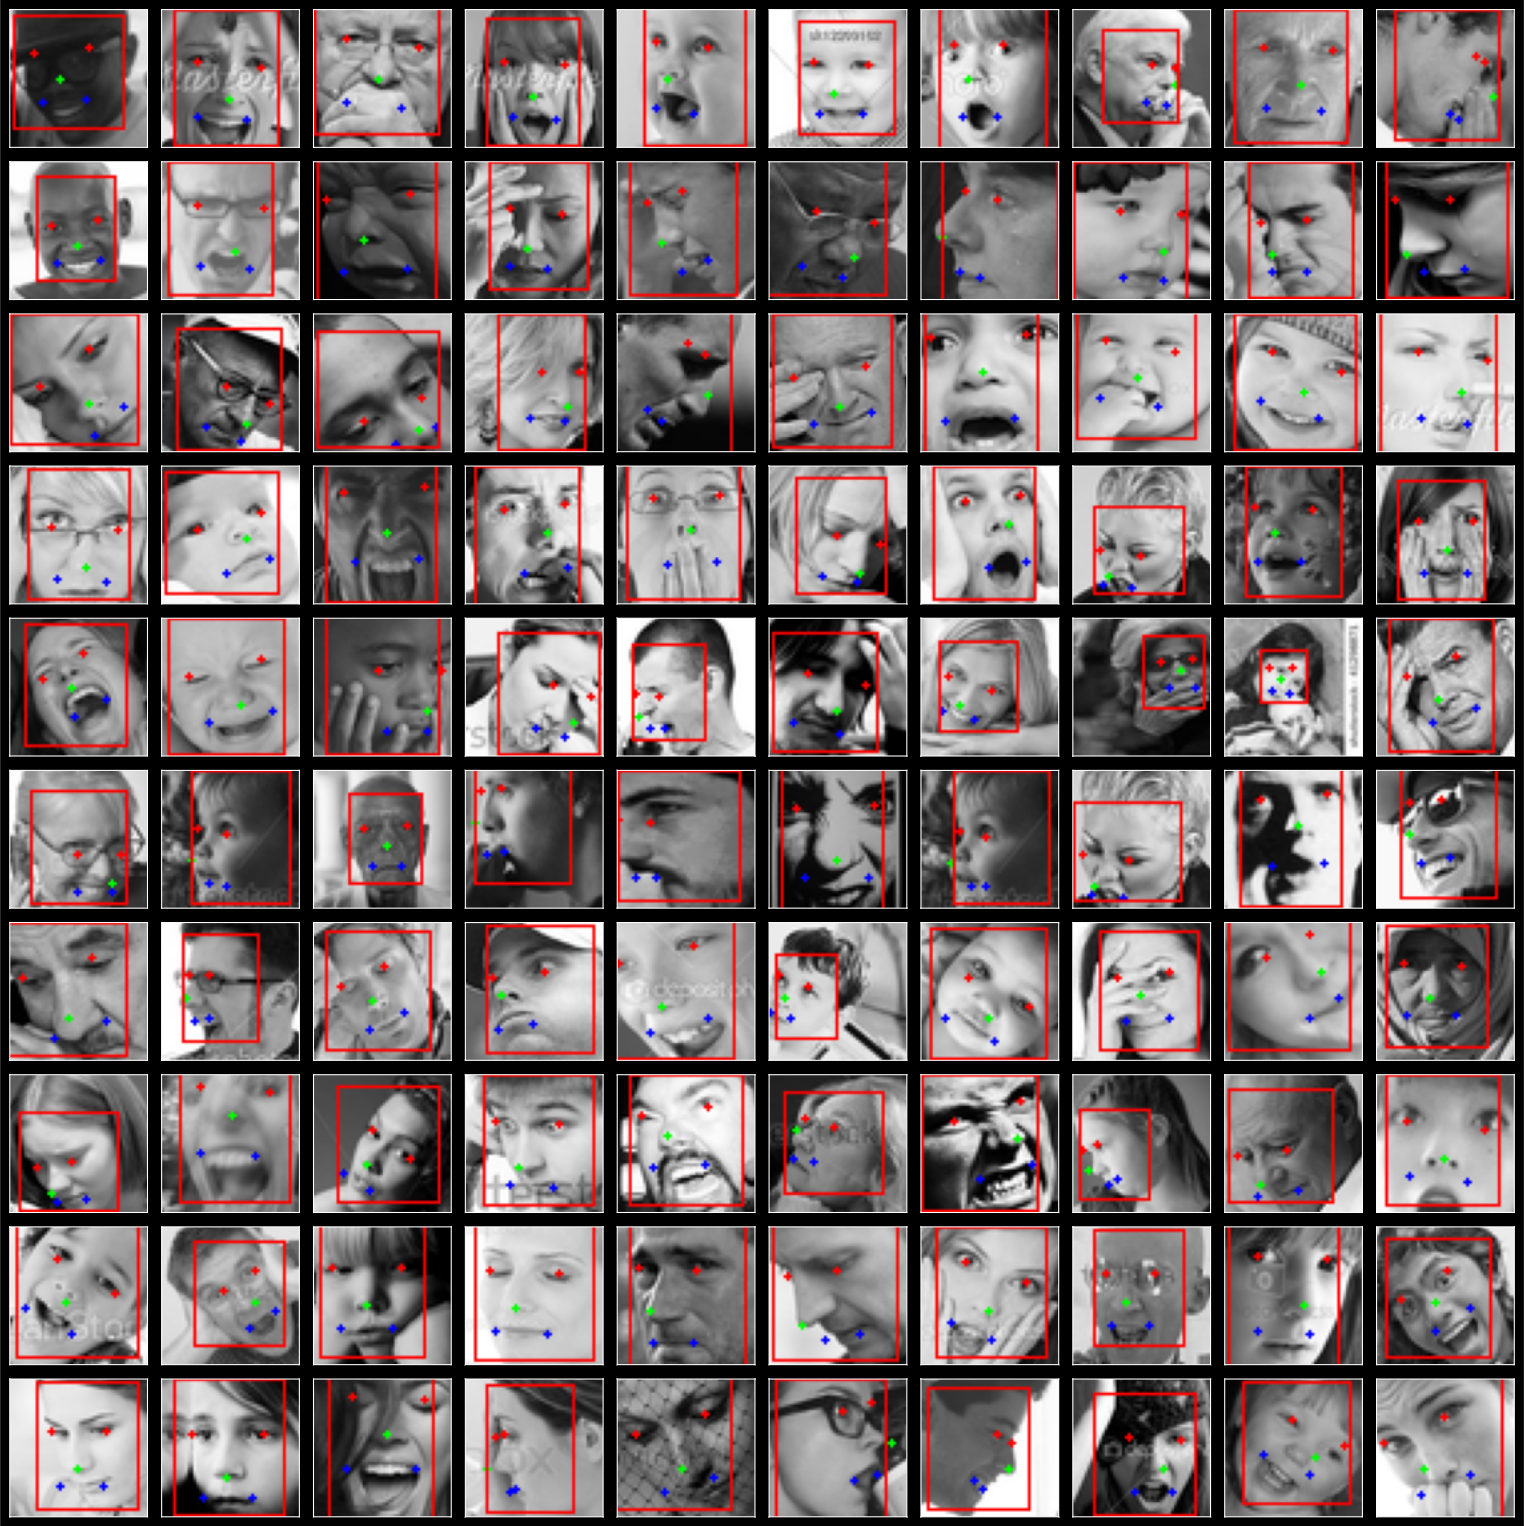
\includegraphics[width=14cm]{gambar/contoh_hasil_retinaface_score50.png}
    \caption{Beberapa Contoh Hasil Deteksi \textit{Facial Landmark} terhadap FER-2013 Menggunakan \textit{RetinaFace} pada ResNet50}
    \label{fig:contohhasilretinaface}
\end{figure}
Berdasarkan Gambar \ref{fig:contohhasilfacealignment} di baris pertama dan kedua, metode \acrshort{fan} sangat presisi dalam memprediksi \textit{facial landmark}. Bahkan berhasil memprediksi \textit{facial landmark} pada objek-objek wajah dengan rotasi yang sangat ekstrem dan/atau halangan yang cukup mengganggu. Namun, pendeteksiannya tidak akurat bahkan sangat berantakan untuk sampel gambar wajah di baris ketiga. Sayangnya, penulis pun tidak dapat menyimpulkan gambar-gambar wajah dengan karakteristik bagaimana yang gagal diprediksi. Oleh karena penulis kesulitan jika harus memeriksa satu per satu hasilnya, maka metode \acrshort{fan} dinilai tidak bisa diandalkan.

Kemudian penulis mencoba meninjau hasil prediksi metode \textit{RetinaFace} dengan ResNet50 yang ditunjukkan pada Gambar \ref{fig:contohhasilretinaface}. Di sini penulis mengambil sampel dari seratus gambar wajah pertama yang berhasil dikenali dan diprediksi dengan skor yang mendekati \textit{threshold}. Hasilnya, prediksi \textit{facial landmark} menggunakan metode ini cukup akurat dan presisi. Disertai kenyataan bahwa entri data terkait yang gagal dikenali tersebar cukup merata pada setiap label emosi, maka metode ini menjadi pilihan penulis yang terbaik dalam mendeteksi \textit{facial landmark}.

\begin{figure}
    \centering
    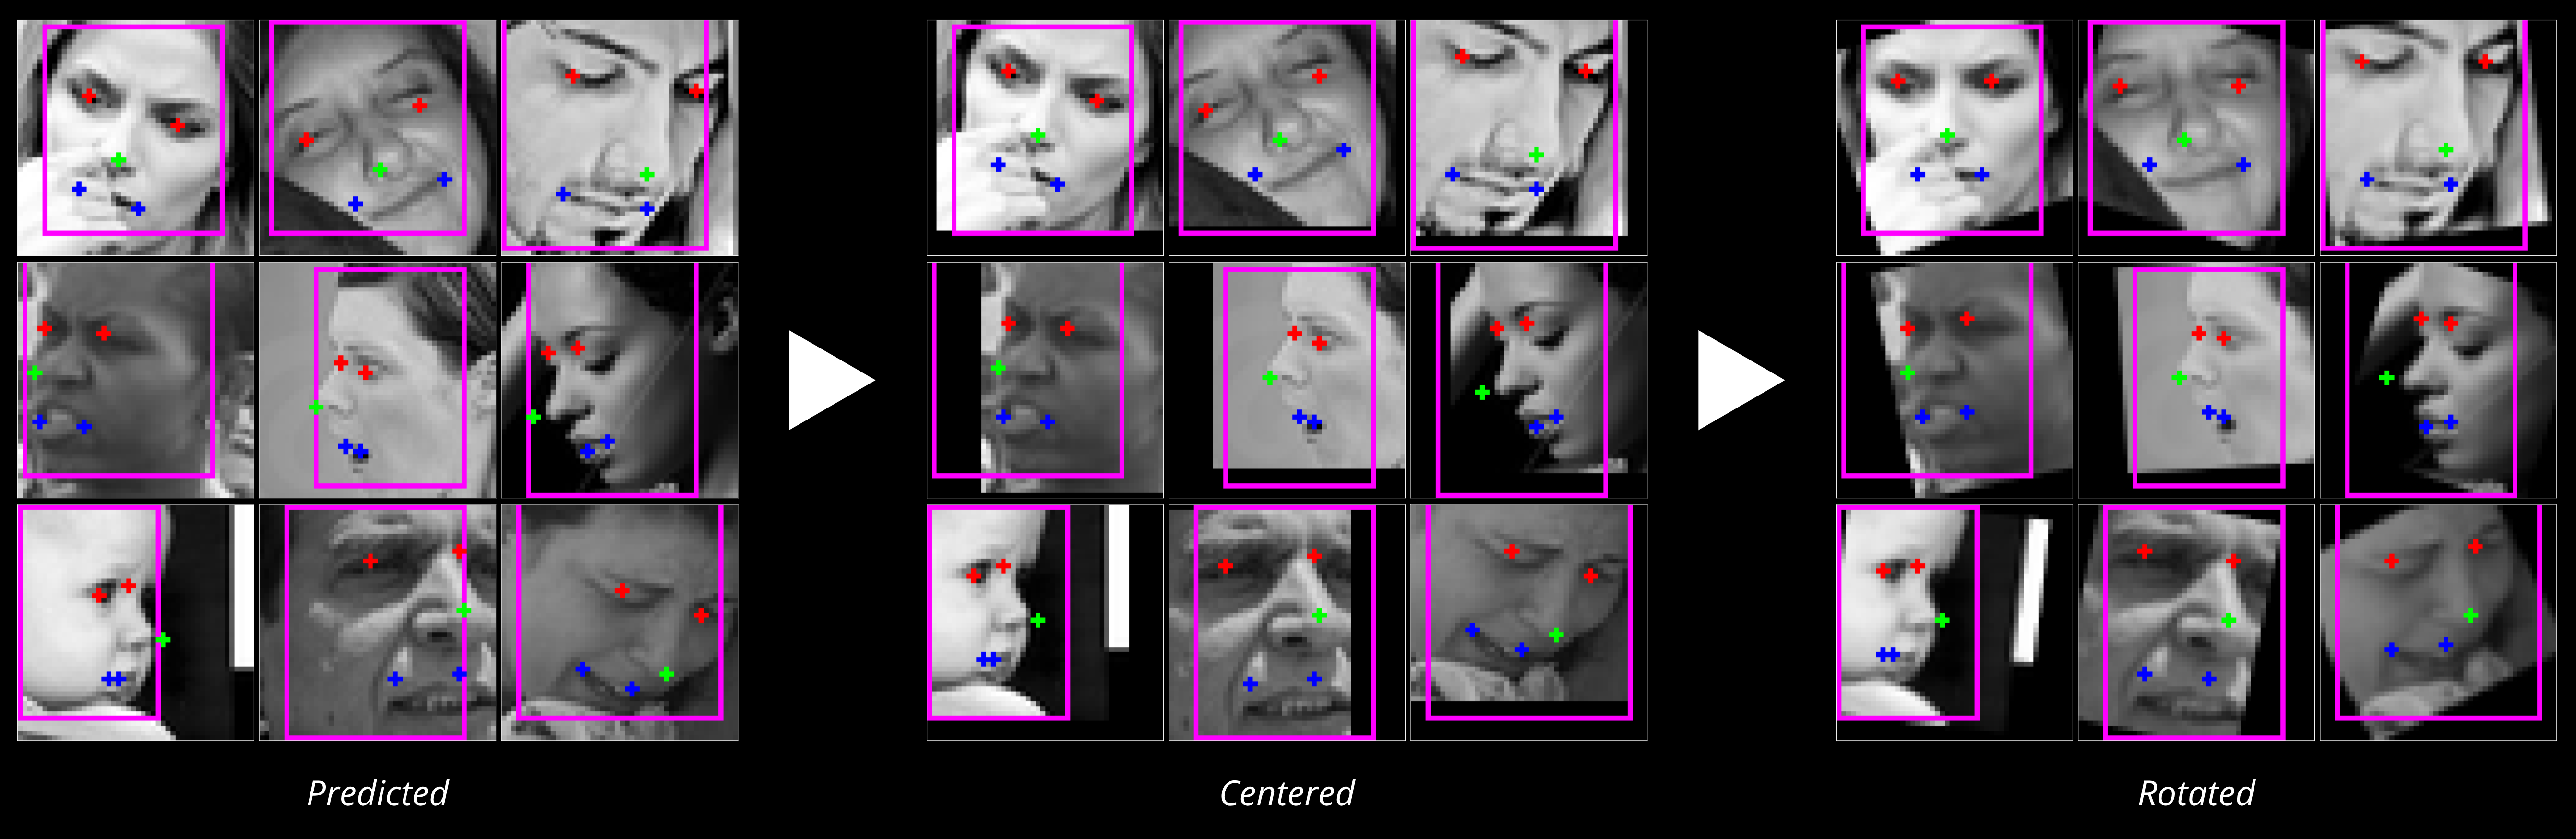
\includegraphics[width=14cm]{gambar/proses_face_alignment.png}
    \caption{Beberapa Contoh Hasil per Subtahap \textit{Face Alignment}}
    \label{fig:prosesfacealignment}
\end{figure}
Tahap ketiga adalah \textit{face alignment}, di mana dilakukan penjajaran setiap objek wajah menggunakan pustaka \textit{opencv} berdasarkan \textit{bounding box} wajah dan \textit{facial landmark} yang bersesuaian. Pertama-tama, sentralisasi setiap objek wajah dilakukan melalui penggeseran seluruh piksel gambar sejauh perpindahan antara titik senter semua \textit{facial landmark} ke titik senter \textit{bounding box} wajah. Lalu perotasian setiap objek wajah dilakukan terhadap titik senter \textit{bounding box} melalui teknik tertentu yang sesuai dengan salah satu dari tiga situasi yang telah didefinisikan. Situasi pertama adalah jika koordinat pada sumbu x tengara hidung berada di tengah-tengah antara tengara sisi kiri dan kanan bibir, maka perotasian dilakukan untuk menjajarkan koordinat pada sumbu y kedua tengara mata. Situasi kedua adalah jika koordinat pada sumbu x tengara hidung berada di kiri terhadap tengara sisi kiri bibir, maka perotasian dilakukan untuk menjajarkan koordinat pada sumbu x tengara mata kanan dan sisi kanan bibir. Situasi ketiga adalah jika koordinat pada sumbu x tengara hidung berada di kanan terhadap tengara sisi kanan bibir, maka perotasian dilakukan untuk menjajarkan koordinat pada sumbu x tengara mata kiri dan sisi kiri bibir. Setiap proses pada tahap ini direpresentasikan ke dalam Gambar \ref{fig:prosesfacealignment}, di mana setiap baris gambar mencontohkan hasil dari masing-masing situasi secara berurutan dari atas ke bawah.

\begin{figure}
    \centering
    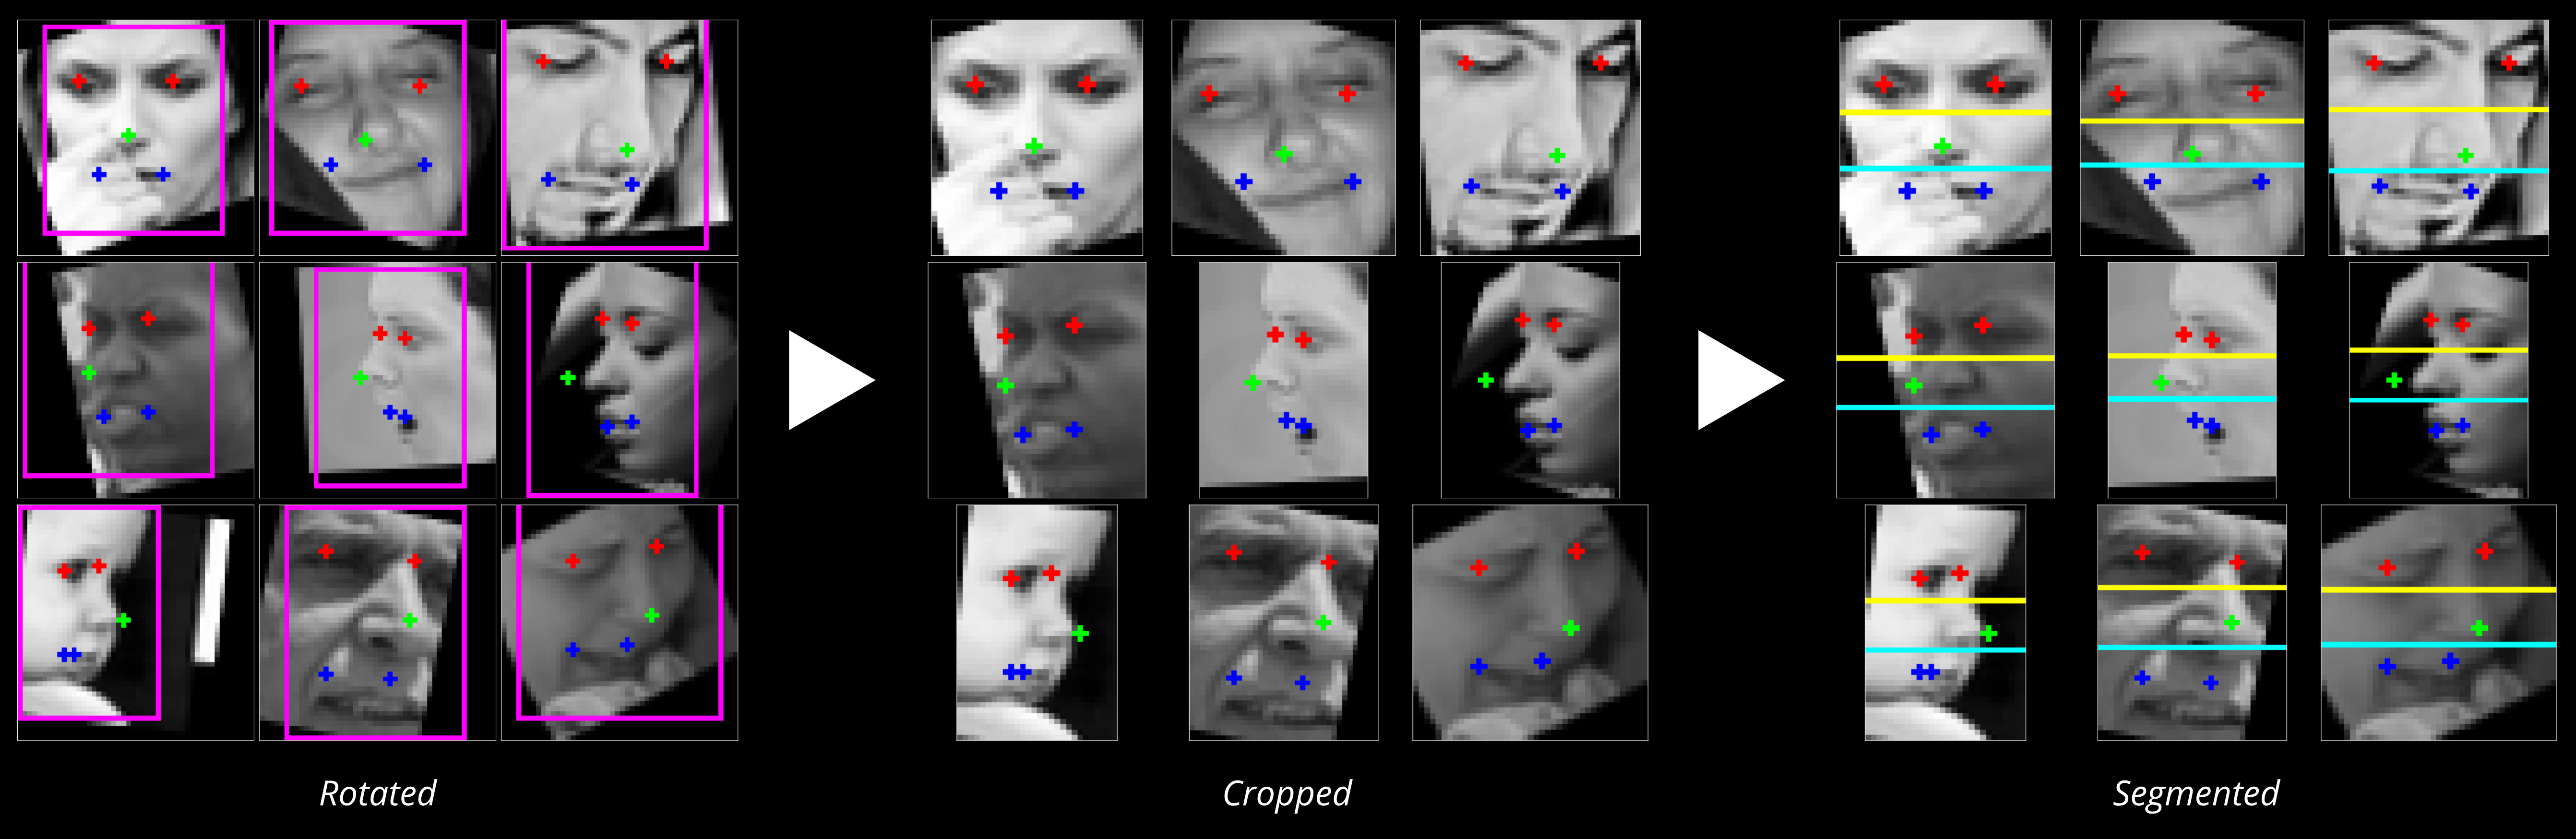
\includegraphics[width=14cm]{gambar/proses_facial_region_segmentation.png}
    \caption{Beberapa Contoh Hasil per Subtahap \textit{\acrlong{frs}}}
    \label{fig:prosesfacialregionsegmentation}
\end{figure}
Tahap keempat adalah \textit{facial region segmentation}, di mana tiap-tiap bagian wajah disegmentasi guna menghasilkan set data sekunder. Pada tahap ini, diusulkan dua konfigurasi segmentasi yang berbeda. Konfigurasi pertama adalah pembagian setiap objek wajah menjadi tiga area, yaitu kedua mata, hidung dan mulut. Sedangkan konfigurasi kedua adalah pembagian dua area yang saling tumpang tindih (\textit{overlapping}), yaitu area kedua mata hingga hidung dan area hidung hingga mulut. Proses segmentasi ini dilakukan dengan memotong gambar sesuai dengan \textit{bounding box}, melakukan kalkulasi ulang untuk tiap-tiap \textit{facial landmark} dan memotong gambar per area yang ditentukan. Setiap area yang dipotong didefinisikan oleh sisi-sisi \textit{bounding box} dan garis horizontal yang melalui titik tengah antar dua area yang bersinggungan. Misalnya untuk area kedua mata, dibatasi oleh sisi atas, kiri dan kanan \textit{bounding box} serta garis horizontal batas area kedua mata dan hidung. Contoh-contoh setiap proses pada tahap ini dapat dilihat pada Gambar \ref{fig:prosesfacialregionsegmentation}.

Secara khusus, melalui algoritma segmentasi yang dikembangkan pada penelitian ini, penulis berupaya menjawab permasalahan segmentasi bagian-bagian wajah pada set data wajah nonfrontal. Yang mana set data tersebut memuat berbagai variasi stuktur wajah yang berbeda \shortcite{islam2018facial3}.

\section{Eksekusi Skenario Pemodelan}
Pada subbab ini, penulis akan menjelaskan proses dan hasil eksperimen secara mendetail untuk setiap skenario pemodelan yang telah direncanakan. Setiap skenario dijalankan sebanyak tiga kali percobaan tanpa mengubah konfigurasi apapun untuk lalu diambil model dengan performa yang terbaik. Penggunaan statistik pada percobaan berulang merupakan solusi tradisional dalam menyimpulkan kinerja model. Meskipun pada dasarnya penulis telah mengeset \textit{seed} untuk setiap \textit{random number generator} ke nilai tertentu, performa model tetap terus berubah pada pengulangan percobaan yang berikutnya.

\subsection{Implementasi \acrshort{cnn} \textit{Baseline}}
\begin{table}[t]
    \caption[Perbandingan Performa Model \textit{Baseline} dengan dan tanpa Augmentasi Data]{Perbandingan Performa Model Baseline dengan dan tanpa Augmentasi Data}
    \label{tab:eksperimenbaseline}
    \begin{tabular}{|L{5.4cm}|C{2.6cm}|C{1.5cm}|C{2.7cm}|}
        \hline
        & Akurasi (\%)$^\bigtriangleup$ & \textit{Epoch} & Waktu (jam)$^\bigtriangledown$ \\
        \hline\hline
        Tanpa data augmentasi & 54,24 & 48 & 0,31 \\
        \hline
        Dengan data augmentasi & 60,27 & 174 & 1,64 \\
        \hline
    \end{tabular}
    \footnotesize
    {\raggedright Akurasi---akurasi model pada \textit{testing}; \textit{Epoch}---banyak \textit{epoch} yang dibutuhkan agar model menjadi optimal; Waktu---waktu yang dibutuhkan agar model menjadi optimal; $^\bigtriangleup$Lebih tinggi lebih baik; $^\bigtriangledown$Lebih rendah lebih baik.}
\end{table}
\begin{figure}[t]
    \centering
    \begin{subfigure}[t]{6.75cm}
        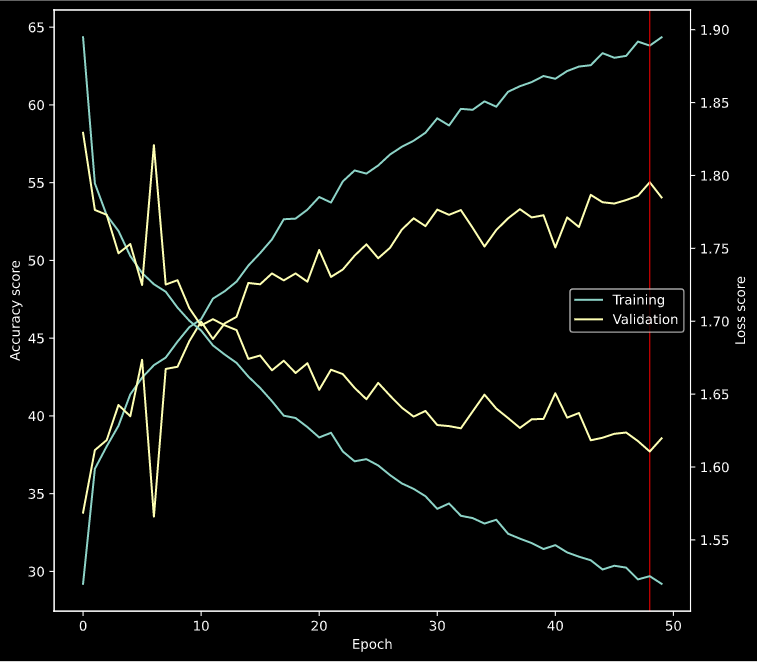
\includegraphics[width=6.75cm]{gambar/eksperimen1_grafik1.png}
        \caption{Grafik Performa Per \textit{Epoch} untuk Model tanpa Augmentasi Data}
        \label{fig:grafikeksperimen1}
    \end{subfigure}
    ~~~
    \begin{subfigure}[t]{6.75cm}
        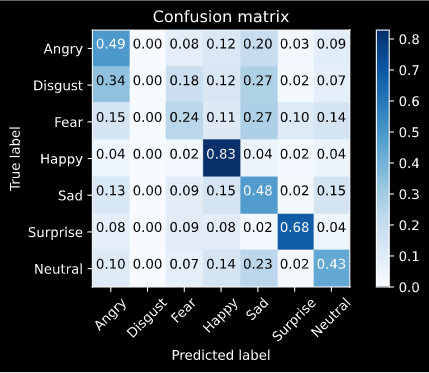
\includegraphics[width=6.75cm]{gambar/eksperimen1_matriks1.png}
        \caption{\textit{Confusion Matrix} Performa Model tanpa Augmentasi Data}
        \label{fig:confusionmatrixeksperimen1}
    \end{subfigure}
    \caption{Performa Model \acrshort{cnn} \textit{Baseline} tanpa Augmentasi Data}
    \label{fig:hasileksperimen1}
\end{figure}
\begin{figure}[!htb]
    \centering
    \begin{subfigure}[t]{6.75cm}
        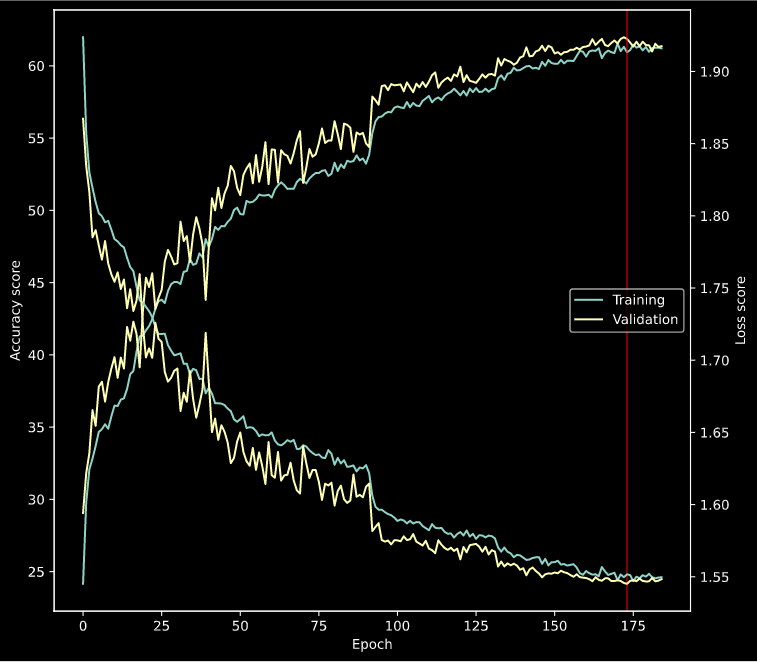
\includegraphics[width=6.75cm]{gambar/eksperimen2_grafik1.png}
        \caption{Grafik Performa Per \textit{Epoch} untuk Model dengan Augmentasi Data}
        \label{fig:grafikeksperimen2}
    \end{subfigure}
    ~~~
    \begin{subfigure}[t]{6.75cm}
        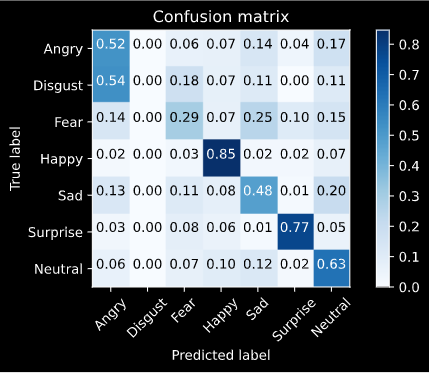
\includegraphics[width=6.75cm]{gambar/eksperimen2_matriks1.png}
        \caption{\textit{Confusion Matrix} Performa Model dengan Augmentasi Data}
        \label{fig:confusionmatrixeksperimen2}
    \end{subfigure}
    \caption{Performa Model \acrshort{cnn} \textit{Baseline} dengan Augmentasi Data}
    \label{fig:hasileksperimen2}
\end{figure}
\begin{figure}[t]
    \centering
    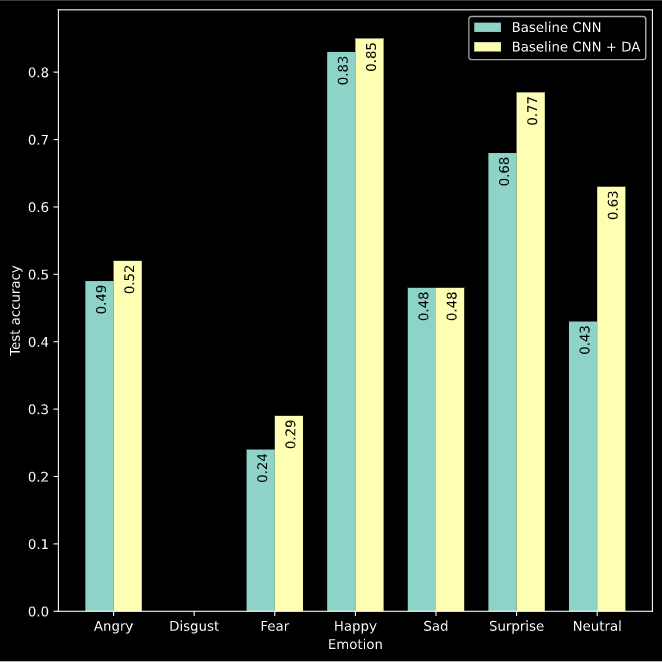
\includegraphics[width=10cm]{gambar/eksperimen1vs2_grafik1.png}
    \caption{Perbandingan Performa Model dengan dan\\tanpa Augmentasi Data Per Kelas Emosi}
    \label{fig:perbandinganeksperimen1dan2}
\end{figure}
Eksperimen dimulai dengan mengimplementasikan model \acrshort{cnn} \textit{baseline} pilihan untuk pengenalan ekspresi wajah pada set data FER-2013. Model yang diklaim dapat mencapai akurasi tes 65,23\% tersebut, berhasil penulis rekonstruksi ulang. Namun, penulis kesulitan bahkan hanya untuk mendekati akurasi tersebut. Penulis menduga terdapat beberapa alasan untuk hal ini. Pertama, yang mana merupakan hal yang paling penting, pembagian distribusi data \textit{training}, \textit{validation} dan \textit{testing} berbeda. Jika pada penelitian \textit{baseline} menggunakan rasio 80:20 untuk data \textit{training} dan \textit{testing}, penulis menggunakan rasio 80:10:10 berturut-turut untuk data \textit{training}, \textit{validation} dan \textit{testing} sesuai dengan \textit{default} dari set data FER-2013 sendiri. Dengan mempertimbangkan bahwa hampir seluruh penelitian pada FER-2013 menggunakan rasio 80:10:10, akan menjadi lebih adil bagi penulis dalam membandingkan hasil metode usulan penulis dengan penelitian lain. Kedua, penelitian \textit{baseline} tidak memerinci bagaimana cara mereka melakukan augmentasi data. Menurut pengamatan penulis, penggunaan teknik augmentasi data dapat meningkatkan performa model pada FER-2013. Seperti yang terlihat pada Tabel \ref{tab:eksperimenbaseline}, augmentasi data telah meningkatkan performa model secara cukup signifikan, yaitu sebesar 6,03\%. Performa model meningkat untuk setiap label emosi kecuali \textit{disgust} dan \textit{sad}. Jika membandingkan \textit{confusion matrix} pada Gambar \ref{fig:confusionmatrixeksperimen1} dan \ref{fig:confusionmatrixeksperimen2}, data berlabel \textit{disgust} malah lebih banyak dikenali sebagai \textit{angry}. Meskipun waktu \textit{training}-nya meningkat sebesar 5,29 kali lipat.

Pada tahap augmentasi data, penulis mengadopsi tiga macam teknik berturut-turut adalah transformasi \textit{affine} acak, \textit{horizontal flipping} acak dan \textit{random erasing}. Khusus untuk eksperimen yang melibatkan \textit{facial region segmentation}, teknik \textit{random erasing} tidak digunakan sebab arsitektur \acrshort{cnn} kesulitan untuk belajar. Sebab memang untuk kasus tertentu, pengombinasian lebih dari dua teknik augmentasi data dapat mempengaruhi kemampuan model dalam generalisasi. Proses augmentasi data ini dilakukan secara berulang per \textit{batch}, atau biasa disebut sebagai \textit{online data augmentation}, agar proses \textit{training} tidak terlalu berat pada komputer berspesifikasi yang telah disebutkan pada bab sebelumnya. Gambar \ref{fig:prosesaugmentasidata} memperlihatkan beberapa contoh untuk setiap proses data augmentasi.
\begin{figure}[t]
    \centering
    \includegraphics[width=14cm]{gambar/proses_augmentasi_data.png}
    \caption{Beberapa Contoh Hasil Per Subtahap \textit{Augmentasi Data}}
    \label{fig:prosesaugmentasidata}
\end{figure}

\begin{figure}[t]
    \centering
    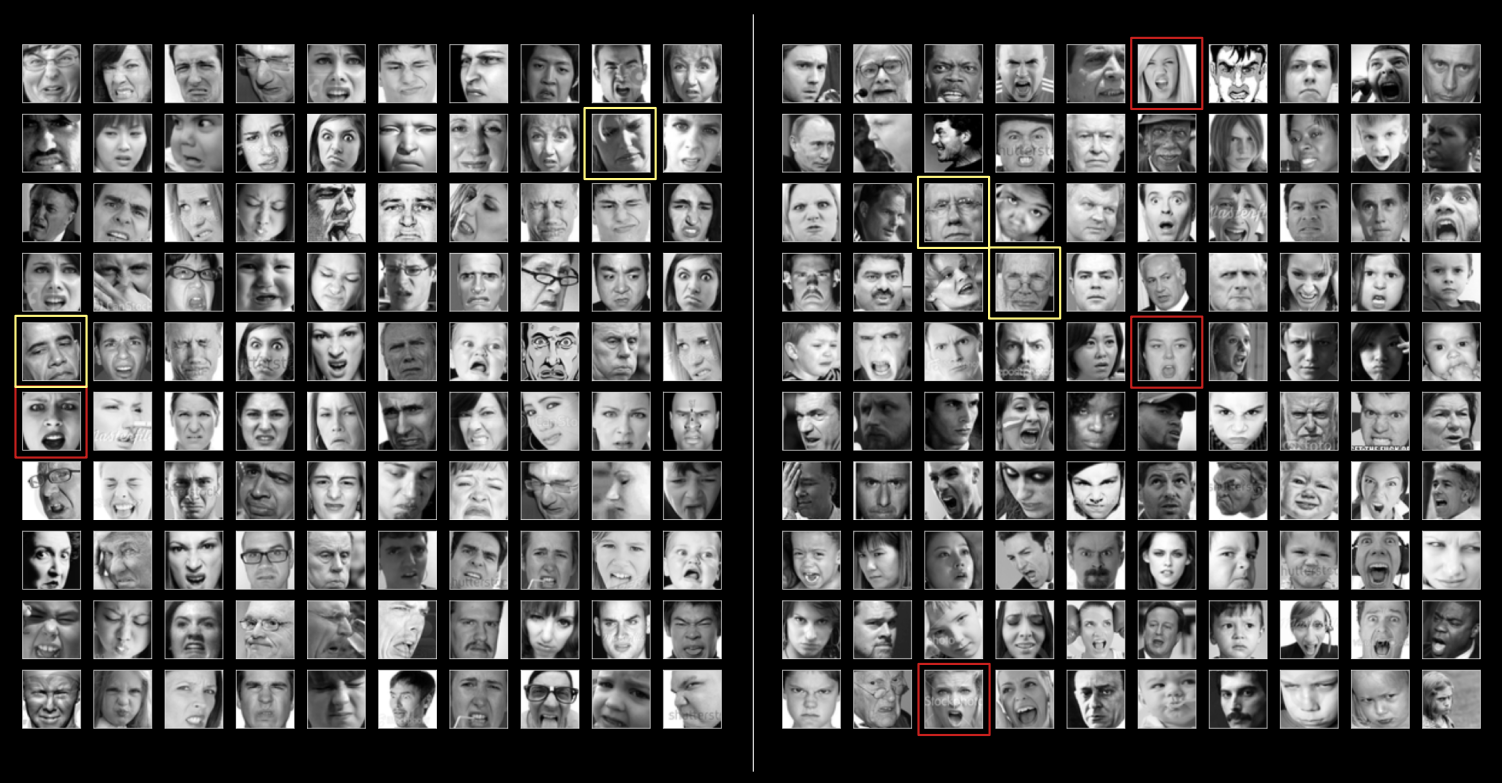
\includegraphics[width=14cm]{gambar/fer2013_disgustvsangry.png}
    \caption{Beberapa Contoh Kemiripan Data Gambar Wajah Berlabel Emosi \textit{Disgust} (Kiri) dan \textit{Angry} (Kanan) pada FER-2013}
    \label{fig:disgustvsangry}
\end{figure}
\begin{figure}[t]
    \centering
    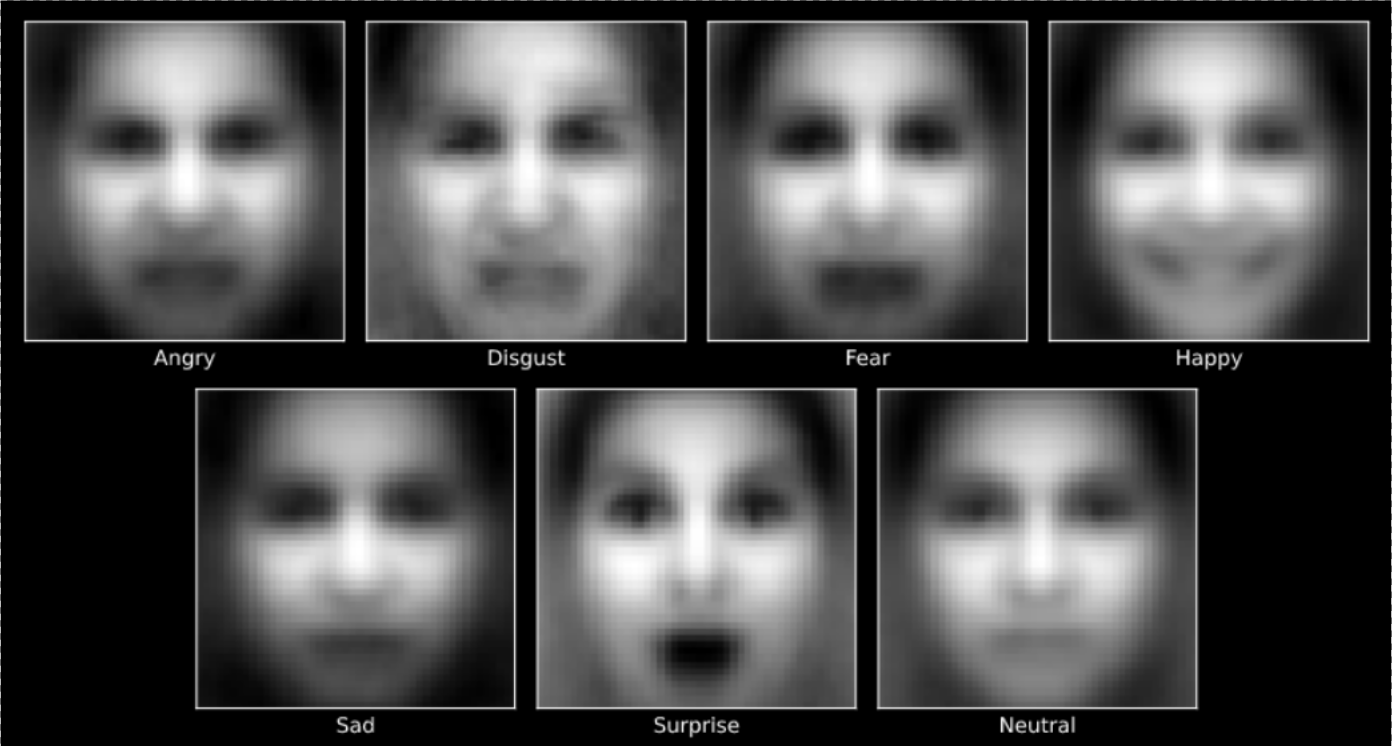
\includegraphics[width=14cm]{gambar/fer2013_rerata_gambar_per_label.png}
    \caption{Rerata Seluruh Data Gambar Wajah pada FER-2013 Per Label Emosi}
    \label{fig:reratagambarfer2013}
\end{figure}
Ada beberapa pertanyaan yang muncul setelah melihat \textit{confusion matrix} pada Gambar \ref{fig:grafikeksperimen2}. Pertama, yang mana merupakan hal yang paling mencolok, model tidak pernah berhasil dalam mengenali emosi berlabel \textit{disgust}. Apakah karena data \textit{training}-nya terlalu sedikit? Lalu jika dilihat secara saksama, emosi \textit{disgust} lebih banyak dikenali sebagai \textit{angry}. Apakah karena emosi \textit{disgust} sulit dibedakan dari \textit{angry}? Untuk itu, penulis melakukan pembandingan beberapa sampel data dari kedua label emosi tersebut yang dapat dilihat pada Gambar \ref{fig:disgustvsangry}. Di sana terlihat beberapa data gambar yang telah ditandai ternyata memang agak sulit untuk dibedakan oleh penulis secara manual sekalipun. Namun hanya dengan ini, penulis tidak bisa serta-merta menyimpulkan bahwa terdapat kesalahan dalam pelabelan set data FER-2013. Kemudian penulis mencoba melakukan pendekatan yang berbeda untuk menjawab persoalan ini, yaitu dengan menghitung rerata gambar wajah per label emosi. Berdasarkan Gambar \ref{fig:reratagambarfer2013}, penulis menyimpulkan bahwa sebenarnya meskipun terdapat beberapa gambar yang terlihat sangat mirip, namun secara keseluruhan data gambar per label masih dapat dibedakan. Kedua, data berlabel \textit{fear} belum mampu seperempatnya dikenali oleh model. Malahan lebih banyak dikenali sebagai emosi \textit{sad}. Sedangkan untuk data berlabel lain \textit{sad} dan \textit{neutral} masih belum mampu dikenali separuhnya. Penulis menduga bahwa hal ini akibat dari kurangnya kompleksitas model \textit{learning}. Oleh karena itu, penulis bersemangat untuk melanjutkan eksperimen ke skenario yang berikutnya. Secara keseluruhan, performa model rekognisi untuk tiap-tiap label emosi mengalami kenaikan. Gambar \ref{fig:perbandinganeksperimen1dan2} merangkum peningkatan tersebut berdasarkan Gambar \ref{fig:confusionmatrixeksperimen1} dan \ref{fig:confusionmatrixeksperimen2}.

\subsection{Modifikasi \acrshort{cnn} \textit{Baseline} Menjadi \acrshort{gcn}}
\begin{figure}[t]
    \centering
    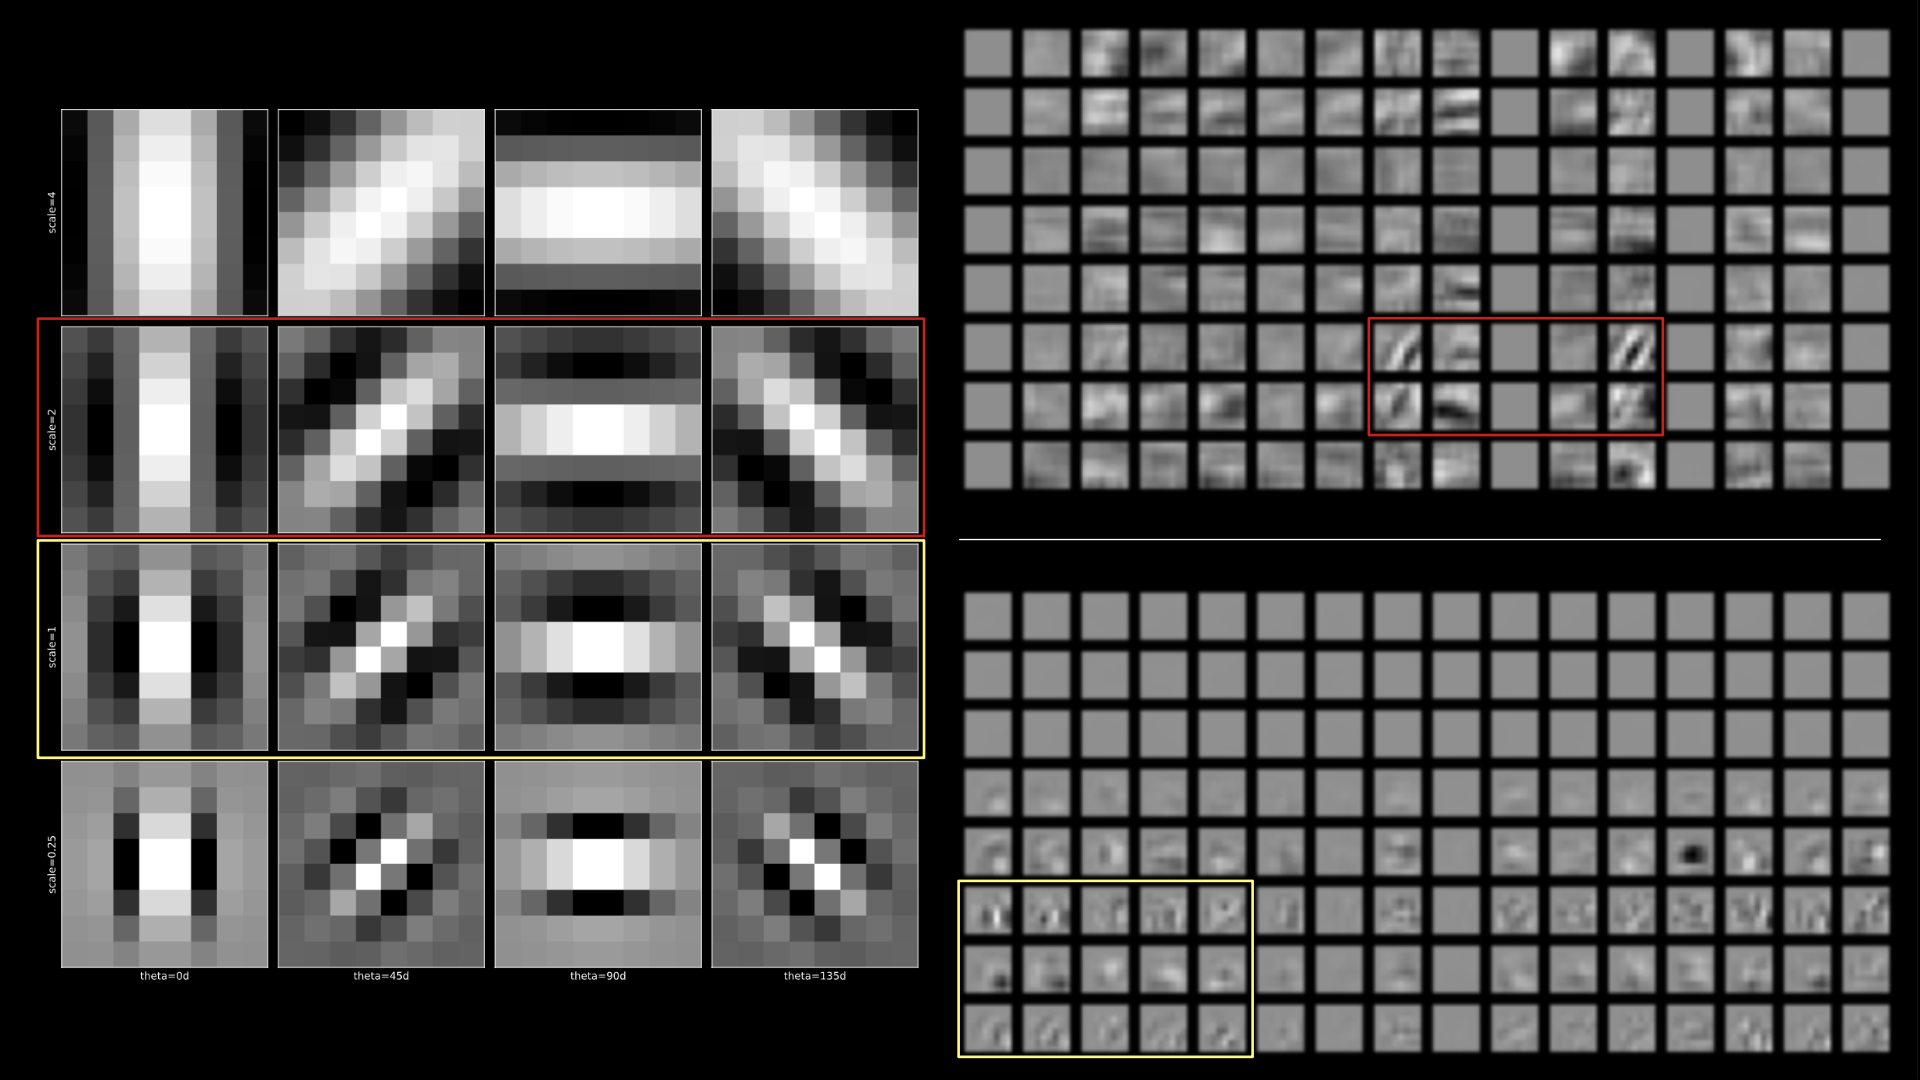
\includegraphics[width=14cm]{gambar/visualisasi_kernel_lapisan8dan9.png}
    \caption{Beberapa Contoh Kemiripan Filter Gabor (Kiri) dengan Kernel dari Lapisan Konvolusi Ke-8 (Kanan Atas) dan Ke-9 (Kanan Bawah) pada Model \acrshort{cnn} \textit{Baseline}}
    \label{fig:visualisasikernel8dan9}
\end{figure}
Pada skenario ke-2 ini, penulis melakukan modifikasi arsitektur \acrshort{cnn} \textit{baseline} menjadi \acrshort{gcn} melalui: 1) pengubahan setiap lapisan konvolusi biasa menjadi lapisan konvolusi Gabor, 2) penambahan sebuah \textit{max layer} sebelum lapisan akhir dan 3) penambahan sebuah lapisan \textit{dense} (\textit{fully connected layer}) di bagian paling akhir dalam arsitektur model.

Pada arsitektur \acrshort{gcn}, terdapat dua parameter tambahan yang perlu ditentukan, yaitu $M$ dan \textit{scale}. $M$ adalah parameter yang menentukan banyaknya variasi rotasi filter Gabor yang akan dipakai dalam rentang 0--180\degree. Jika $M = 1$, maka hanya sebuah filter Gabor pada sudut 0\degree\ yang dipakai. Jika $M > 2$, maka filter Gabor yang dipakai adalah sebanyak $M$ buah meliputi sebuah filter Gabor pada sudut 0\degree\ ditambah $M - 1$ buah filter Gabor pada rotasi yang dihitung secara kumulatif menurut $\theta = (i/M) \times 180\degree$ di mana $i$ adalah indeks urutan filter Gabor yang dimulai dari $i = 1$. Sedangkan \textit{scale} adalah skala filter Gabor relatif terhadap ukuran kernel yang dipakai pada setiap lapisan konvolusi, yaitu $8 \times 8$. Dari enam belas lapisan konvolusi pada arsitektur \textit{baseline}, penulis mengelompokkannya menjadi empat grup secara berurutan. Kemudian penulis melakukan \textit{training} pada model \acrshort{cnn} \textit{baseline} yang telah diubah menjadi \acrshort{gcn} melalui pencacahan konfigurasi parameter $M$ dalam rentang nilai 1--4 dan \textit{scale} dalam rentang nilai yang sama. Dari situ penulis dapat menyimpulkan bahwa parameter yang optimal untuk kasus ini adalah $M = 4$ dengan $\text{scale} = 2$ untuk lapisan konvolusi ke-1 hingga ke-8 dan $\text{scale} = 1$ untuk lapisan konvolusi yang lain. Hal ini dapat dijelaskan melalui visualisasi kernel pada setiap lapisan konvolusi, di mana kernel pada lapisan konvolusi ke-8 ke bawah mirip dengan filter Gabor pada $\text{scale} = 2$ dan kernel pada lapisan konvolusi ke-9 ke atas mirip dengan filter Gabor pada $\text{scale} = 1$. Pada Gambar \ref{fig:visualisasikernel8dan9} diperlihatkan beberapa contoh kemiripan tersebut. Pada bagian kiri, ditampilkan empat baris filter Gabor dengan parameter \textit{scale} yang berbeda pada empat rotasi yang berbeda. Pada bagian kanan, dari atas ke bawah, menunjukkan separuh kernel dari lapisan konvolusi ke-8 dan ke-9 secara berurutan.

\begin{table}[!t]
    \caption[Perbandingan Performa Model \acrshort{cnn} \textit{Baseline} dan \acrshort{gcn}]{Perbandingan Performa Model \acrshort{cnn} Baseline dan \acrshort{gcn}}
    \label{tab:eksperimengcn}
    \begin{tabular}{|L{5.4cm}|C{2.6cm}|C{1.5cm}|C{2.7cm}|}
        \hline
        & Akurasi (\%)$^\bigtriangleup$ & \textit{Epoch} & Waktu (jam)$^\bigtriangledown$ \\
        \hline\hline
        Model \acrshort{cnn} \textit{baseline} & 60,27 & 174 & 1,64 \\
        \hline
        Model \acrshort{gcn} & 63,51 & 150 & 7,95 \\
        \hline
    \end{tabular}
    \footnotesize
    {\raggedright Akurasi---akurasi model pada \textit{testing}; \textit{Epoch}---banyak \textit{epoch} yang dibutuhkan agar model menjadi optimal; Waktu---waktu yang dibutuhkan agar model menjadi optimal; $^\bigtriangleup$Lebih tinggi lebih baik; $^\bigtriangledown$Lebih rendah lebih baik.}
\end{table}
\begin{figure}[ht]
    \centering
    \begin{subfigure}[t]{6.75cm}
        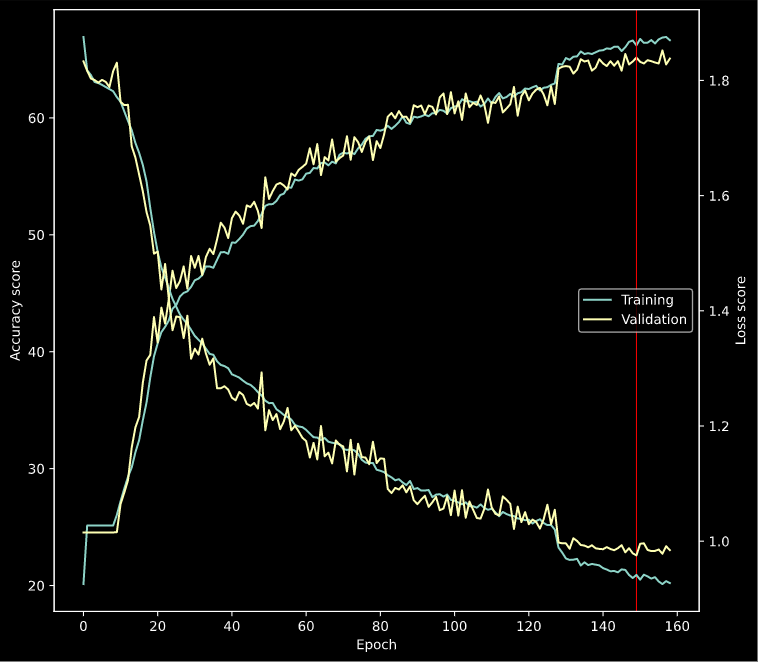
\includegraphics[width=6.75cm]{gambar/eksperimen3_grafik1.png}
        \caption{Grafik Performa Per \textit{Epoch} untuk Model \acrshort{gcn}}
        \label{fig:grafikeksperimen3}
    \end{subfigure}
    ~~~
    \begin{subfigure}[t]{6.75cm}
        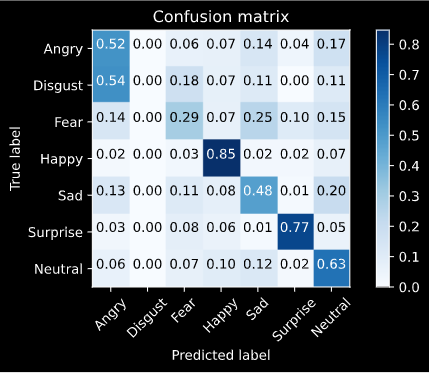
\includegraphics[width=6.75cm]{gambar/eksperimen2_matriks1.png}
        \caption{\textit{Confusion Matrix} Performa Model \acrshort{gcn}}
        \label{fig:confusionmatrixeksperimen3}
    \end{subfigure}
    \caption{Performa Model \acrshort{gcn}}
    \label{fig:hasileksperimen3}
\end{figure}
Dari eksperimen ini dibuktikan bahwa model \acrshort{gcn}, yang merupakan hasil modifikasi dari \acrshort{cnn} \textit{baseline}, memiliki performa yang lebih unggul dari pendahulunya. Sebagaimana yang terangkum dalam Tabel \ref{tab:eksperimengcn}, performa model meningkat sebesar 3,24\% disertai oleh peningkatan waktu \textit{training} sebesar 4,84 kali lipat. Di sisi lain, banyak \textit{epoch} yang harus dilalui untuk melatih model \acrshort{gcn} lebih rendah daripada sebelumnya untuk \textit{batch size} yang sama.

Sebelum membahas lebih lanjut mengenai perbandingan performa kedua model, ada dua hal yang menarik bagi penulis ketika membandingkan grafik log performa model pada Gambar \ref{fig:grafikeksperimen2} dan \ref{fig:grafikeksperimen3}. Pertama, melalui pengamatan penulis pada pengubahan parameter $M$, penggunaan arsitektur model \acrshort{gcn} selalu dimulai dengan grafik akurasi untuk \textit{training} dan \textit{validation} yang sama sekali konstan pada \textit{epoch} ke-1 hingga ke-10. Sementara itu, grafik \textit{loss} untuk \textit{training} dan \textit{validation} selalu mengalami perbaikan. Baru pada \textit{epoch} ke-10 hingga ke-25, tiap-tiap grafik mengalami perbaikan yang sangat signifikan. Sedangkan grafik log performa model yang sebelumnya relatif lebih halus setelah \textit{epoch} ke-5. Hal ini menerangkan bahwa pengenaan filter Gabor pada lapisan konvolusi \acrshort{cnn} menyulitkan mesin untuk belajar, namun memberikan wawasan yang lebih baik dalam rekognisi kelas emosi. Kedua, yang mana mengherankan penulis, grafik performa \textit{validation} hampir selalu lebih baik daripada grafik performa \textit{training} hingga \textit{epoch} tertentu di mana terlihat loncatan peningkatan yang cukup dengan jelas sesaat setelah grafik performa \textit{training} relatif mulai stabil. Jika dibandingkan dengan grafik log performa model yang paling awal pada Gambar \ref{fig:grafikeksperimen1}, hal ini menyatakan bagaimana data augmentasi dan penggunaan \textit{Gabor convolutional layer} dapat meningkatkan kemampuan generalisasi model rekognisi. Adapun kejadian di mana grafik \textit{validation} mulai konstan setelah mengalami loncatan peningkatan yang signifikan, menjelaskan bahwa hal ini terjadi akibat penulis menggunakan teknik pengecilan parameter \textit{learning rate} menggunakan fungsi \textit{reduce learning rate on plateau} dalam \textit{training} dengan faktor pengali sebesar $\sqrt{0,1}$ ketika menemukan bahwa tidak ada peningkatan senilai tertentu pada grafik \textit{validation loss} dalam sepuluh \textit{epoch} terakhir.

\begin{figure}[t]
    \centering
    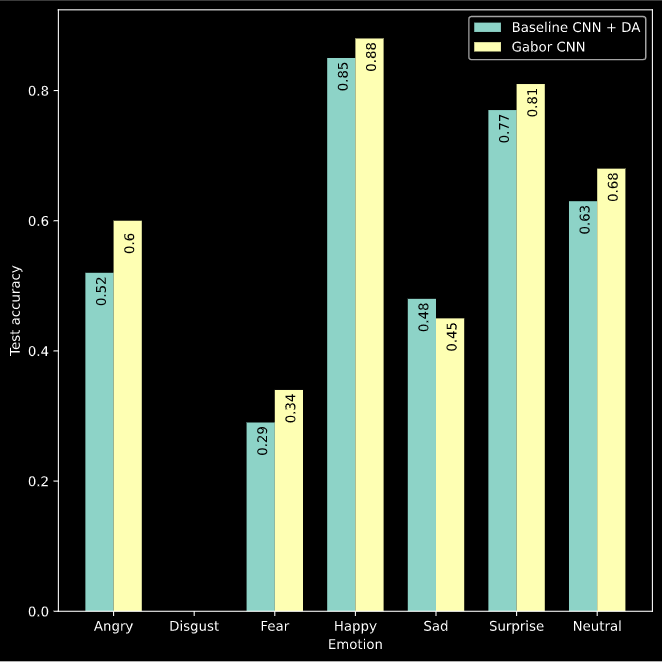
\includegraphics[width=10cm]{gambar/eksperimen2vs3_grafik1.png}
    \caption{Perbandingan Performa Model \acrshort{cnn} \textit{Baseline}\\dan \acrshort{gcn} Per Kelas Emosi}
    \label{fig:perbandinganeksperimen2dan3}
\end{figure}
Secara umum, pengadopsian arsitektur \acrshort{gcn} telah berhasil meningkatkan performa model rekognisi per kelas emosi, seperti yang diperlihatkan pada Gambar \ref{fig:perbandinganeksperimen2dan3}. Performa model meningkat untuk setiap label emosi kecuali \textit{disgust} dan \textit{fear}. Berulang lagi tidak ada perbaikan apapun dalam pengenalan emosi \textit{disgust}. Bahkan jika membandingkan \textit{confusion matrix} pada Gambar \ref{fig:confusionmatrixeksperimen2} dan \ref{fig:confusionmatrixeksperimen3}, data berlabel \textit{disgust} malah lebih banyak lagi dikenali sebagai \textit{angry}. Sehingga penulis berakhir pada kesimpulan bahwa ketimpangan yang sangat jelas terjadi pada banyak data berlabel emosi \textit{disgust} telah menyebabkan kegagalan model dalam mengenali emosi tersebut. Sementara kemampuan model dalam mengenali emosi \textit{sad} menjadi sedikit berkurang.

\subsection{Modifikasi \acrshort{gcn} Menjadi \textit{Ensemble} \acrshort{gcns}}
Pada skenario ini, penulis mencoba membangun \textit{ensemble network} menggunakan dua teknik yang berbeda. Teknik yang pertama merupakan teknik \textit{ensemble} konvensional, yaitu penggabungan hasil prediksi secara terpisah dari setiap model yang dilatih menggunakan bagian wajah tertentu. Hasil prediksi akhir untuk sebuah input gambar baru dihitung menggunakan rumus statistik tertentu, yaitu \textit{simple average} dan \textit{weighted average}. \textit{Simple average} diperoleh melalui operasi perhitungan rata-rata biasa pada (\ref{equ:average}),
\begin{equation}
    \bar{y} = \frac{y_{\text{i}} + y_{\text{j}}}{2}
    \label{equ:average}
\end{equation}
sedangkan \textit{weighted average} diperoleh dari (\ref{equ:waverage}),
\begin{equation}
    \bar{y} = \frac{y_{\text{i}} * a_{\text{i}} + y_{\text{j}} * a_{\text{j}}}{a_{\text{i}} + a_{\text{i}}}
    \label{equ:waverage}
\end{equation}
di mana $y$ adalah larik probabilitas berdimensi $1 \times 7$ hasil prediksi sebuah input baru dan $a$ adalah akurasi tes untuk masing-masing model $i$ dan $j$ yang berbeda. Sejujurnya, alangkah lebih baik jika \textit{weighted average} dihitung dengan mempertimbangkan akurasi tes per kelas pada \textit{confusion matrix}. Namun penulis kesulitan menghitungnya, sebab model sama sekali tidak bisa memprediksi data berlabel \textit{disgust}. Sementara teknik yang kedua bekerja dengan menggabungkan arsitektur jaringan sebanyak $n$ menjadi jaringan bertingkat (\textit{cascaded network}), di mana $n$ adalah banyak bagian wajah yang disegmentasi.

Sebelum membahas hasil eksperimen pada skenario ini, perlu diketahui bahwa kali ini penulis meninggalkan fungsi \textit{reduce learning rate on plateau}. Karena menurut hasil pengamatan penulis, proses \textit{training} pada skenario ini relatif lambat dan kurang stabil. Sehingga jika penulis tetap menggunakan fungsi tersebut, proses \textit{training} hingga mencapai optimal akan sangat lambat akibat beberapa kali pengecilan \textit{learning rate} dalam rentang waktu yang sebentar.

\begin{table}[t]
    \caption{Perbandingan Performa Berbagai Kombinasi Model \textit{Ensemble} \acrshort{gcns}}
    \label{tab:eksperimengcnfrs}
    \begin{tabular}{|C{2.3cm}|C{1cm}|C{1cm}|C{1.2cm}|C{1.8cm}|C{1.8cm}|C{1.8cm}|}
        \hline
        \multicolumn{1}{|c|}{\multirow{3}{*}{Fitur}} & \multicolumn{2}{c|}{\multirow{3}{*}{Waktu (jam)$^\bigtriangledown$}} & \multicolumn{1}{c|}{\multirow{3}{*}{\textit{Epoch}}} & \multicolumn{3}{c|}{Akurasi \textit{Testing} (\%)$^\bigtriangleup$} \\
        \cline{5-7}
        & \multicolumn{2}{c|}{} &  & \multirow{2}{*}{\textit{Single}} & \textit{Simple Average} & \textit{Weighted Average} \\
        \hline\hline
        \multirow{2}{*}{EN + NM} & 4,17 & \multirow{2}{*}{8,87} & 124 & 58,09 & \multirow{2}{*}{62,20} & \multirow{2}{*}{62,20} \\
        \cline{2-2}\cline{4-5}
        & 4,70 &  & 141 & 58,06 &  &  \\
        \hline
        \multirow{3}{*}{E + N + M} & 3,44 & \multirow{3}{*}{10,34} & 153 & 17,41 & \multirow{3}{*}{44,10} & \multirow{3}{*}{53,22} \\
        \cline{2-2}\cline{4-5}
        & 4,05 &  & 181 & 25,45 &  &  \\
        \cline{2-2}\cline{4-5}
        & 2,85 &  & 129 & 53,88 &  &  \\
        \hline
        E + N & \multirow{3}{*}{Ibid.} & 7,49 & \multicolumn{2}{c|}{\multirow{3}{*}{Ibid.}} & 17,74 & 17,62 \\
        \cline{1-1}\cline{3-3}\cline{6-7}
        N + M &  & 6,90 & \multicolumn{2}{c|}{} & 52,77 & 53,61 \\
        \cline{1-1}\cline{3-3}\cline{6-7}
        E + M &  & 6,29 & \multicolumn{2}{c|}{} & 44,91 & 53,28 \\
        \hline\hline
        EN + NM (\textit{concat.}) & \multicolumn{2}{c|}{\multirow{2}{*}{7,34}} & \multirow{2}{*}{103} & \multirow{2}{*}{59,71} & \multicolumn{2}{c|}{\multirow{4}{*}{-}} \\
        \cline{1-5}
        E + N + M (\textit{concat.}) & \multicolumn{2}{c|}{\multirow{2}{*}{8,36}} & \multirow{2}{*}{131} & \multirow{2}{*}{54,12} & \multicolumn{2}{c|}{} \\
        \hline\hline
        ENM & \multicolumn{2}{c|}{6,80} & 131 & 62,08 & \multicolumn{2}{c|}{-} \\
        \hline
    \end{tabular}
    \footnotesize
    {\raggedright E---(\textit{Eyes}) area bagian kedua mata; N---(\textit{Nose}) area bagian hidung; M---(\textit{Mouth}) area bagian mulut;\\
    \textit{Epoch}---banyak \textit{epoch} yang dibutuhkan agar model menjadi optimal; Waktu---waktu yang dibutuhkan agar model menjadi optimal; $^\bigtriangleup$Lebih tinggi lebih baik; $^\bigtriangledown$Lebih rendah lebih baik.}
\end{table}
\begin{figure}[t]
    \centering
    \begin{subfigure}[t]{6.75cm}
        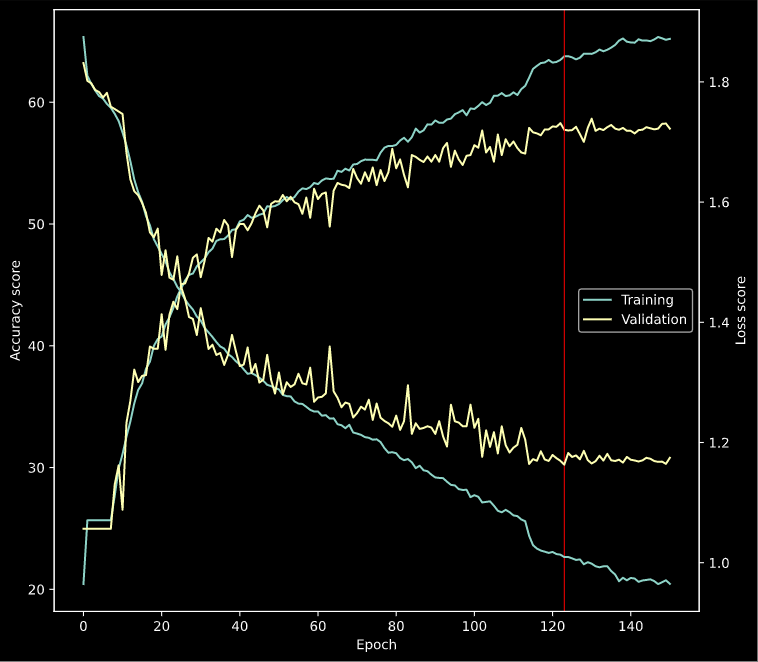
\includegraphics[width=6.75cm]{gambar/eksperimen4b1_grafik1.png}
        \caption{Grafik Performa Per \textit{Epoch} untuk Model EN}
        \label{fig:grafikeksperimen4b11}
    \end{subfigure}
    ~~~
    \begin{subfigure}[t]{6.75cm}
        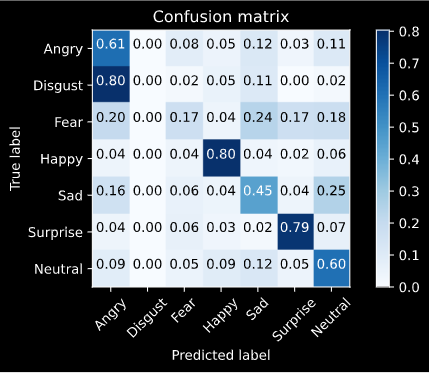
\includegraphics[width=6.75cm]{gambar/eksperimen4b1_matriks1.png}
        \caption{\textit{Confusion Matrix} Performa Model EN}
        \label{fig:confusionmatrixeksperimen4b11}
    \end{subfigure}
    ~~~
    \begin{subfigure}[t]{6.75cm}
        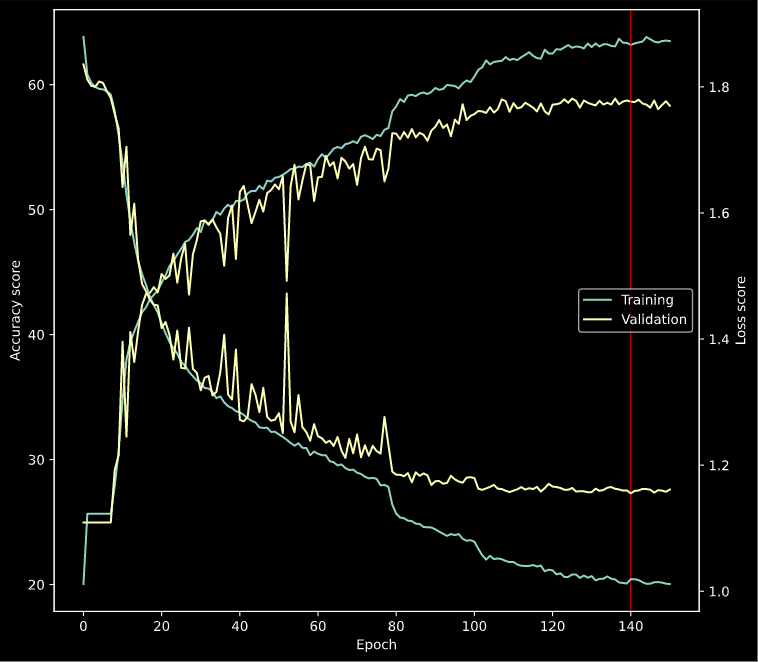
\includegraphics[width=6.75cm]{gambar/eksperimen4b1_grafik2.png}
        \caption{Grafik Performa Per \textit{Epoch} untuk Model NM}
        \label{fig:grafikeksperimen4b12}
    \end{subfigure}
    ~~~
    \begin{subfigure}[t]{6.75cm}
        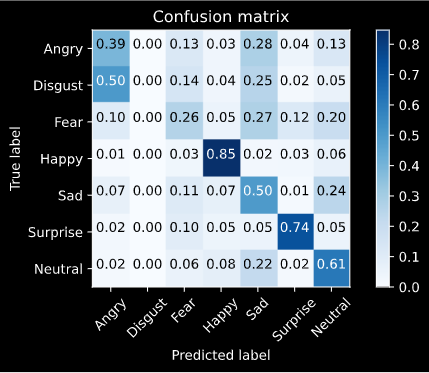
\includegraphics[width=6.75cm]{gambar/eksperimen4b1_matriks2.png}
        \caption{\textit{Confusion Matrix} Performa Model NM}
        \label{fig:confusionmatrixeksperimen4b12}
    \end{subfigure}
    \caption{Performa Model \acrshort{gcns} Menggunakan Fitur EN + NM}
    \label{fig:hasileksperimen4b1}
\end{figure}
\begin{figure}[t]
    \ContinuedFloat
    \centering
    \begin{subfigure}[t]{6.75cm}
        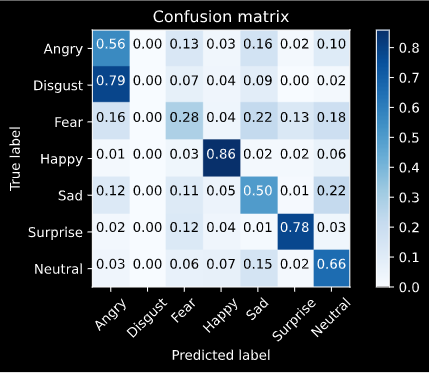
\includegraphics[width=6.75cm]{gambar/eksperimen4b1_matriks3.png}
        \caption{\textit{Confusion Matrix} Performa Model EN + NM Berdasarkan Perhitungan \textit{Simple Average}}
        \label{fig:confusionmatrixeksperimen4b13}
    \end{subfigure}
    ~~~
    \begin{subfigure}[t]{6.75cm}
        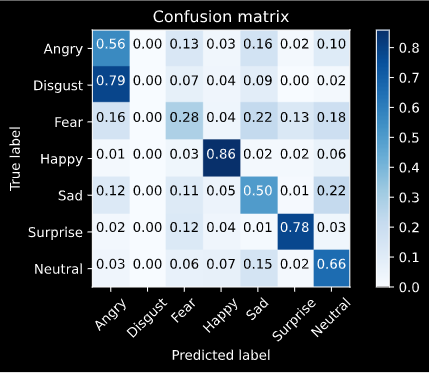
\includegraphics[width=6.75cm]{gambar/eksperimen4b1_matriks4.png}
        \caption{\textit{Confusion Matrix} Performa Model EN + NM Berdasarkan Perhitungan \textit{Weighted Average}}
        \label{fig:confusionmatrixeksperimen4b14}
    \end{subfigure}
    \caption{Performa Model \acrshort{gcns} Menggunakan Fitur EN + NM (Lanjutan)}
\end{figure}
Secara khusus, salah satu tujuan dari skenario ini adalah menjawab sebuah \textit{future work} penelitian terkait demi mengembangkan model rekognisi yang andal menggunakan teknik \acrshort{frs} untuk mampu mengenali emosi dari gambar wajah manusia yang diputar pada sudut berapa pun \shortcite{islam2018facial2}. Hasil dari tiap-tiap eksperimen pada skenario ini terangkum pada Tabel \ref{tab:eksperimengcnfrs}. Pada kolom akurasi \textit{testing}, terlihat bahwa pemodelan menggunakan set data hasil \acrshort{frs} dua bagian wajah (EN + NM) memiliki akurasi yang paling tinggi; jauh lebih baik daripada pemodelan menggunakan tiga bagian wajah (E + N + M) dan kombinasi dua-dua (E + N, N + M dan E + M), baik menggunakan teknik \textit{ensemble} yang pertama maupun yang kedua. Kendati pun akurasinya masih lebih rendah ketimbang model yang dilatih tanpa memanfaatkan teknik \acrshort{frs} (model terbaik pada skenario sebelumnya), namun penurunannya hanya sebesar 1,31\%. Sementara pemodelan menggunakan tiga area wajah dan kombinasi dua-dua tidak bisa diandalkan, bahkan performanya jauh lebih rendah daripada model \textit{baseline}.

Lebih jauhnya, jika ditilik setiap \emph{confusion matrix} yang ditunjukkan pada Gambar \ref{fig:confusionmatrixeksperimen4b11}--\ref{fig:confusionmatrixeksperimen4b8}, maka dapat disimpulkan beberapa poin. Dalam membandingkan masing-masing dari performa model EN dan NM, tampak bahwa model EN memiliki akurasi yang lebih tinggi pada pengenalan emosi \textit{angry} dan \textit{surprise}. Untuk pengenalan emosi \textit{angry}, model EN jauh lebih baik dari model NM dengan selisih 22\%. Sehingga jelas bahwa emosi \textit{angry} lebih mudah dikenali menggunakan bagian wajah atas manusia. Sedangkan model NM relatif sedikit lebih baik pada sisanya. Khusus untuk \textit{disgust}, model EN lebih banyak melakukan kesalahan prediksi sebagai \textit{angry} dengan selisih 30\%. Hal ini menjelaskan bahwa emosi \textit{disgust} lebih sulit dikenali menggunakan bagian wajah atas manusia. Untuk emosi \textit{fear}, dapat disimpulkan bahwa emosi ini lebih sulit dikenali dengan melihat bagian atas dan bawah wajah secara terpisah.

Di sisi lain, performa model EN + NM dalam perhitungan dua teknik rerata memberikan \textit{confusion matrix} yang tepat sama seperti yang terlihat pada Gambar \ref{fig:confusionmatrixeksperimen4b13} dan \ref{fig:confusionmatrixeksperimen4b14}. Untuk setiap label emosi, kombinasi kedua model ini mampu memberikan nilai akurasi yang sedikit lebih baik dibandingkan model NM. Namun untuk label \textit{angry}, akurasinya 5\% lebih rendah daripada model EN. Sementara penyimpangan prediksi emosi \textit{disgust} mendekati kemampuan model EN.

\begin{figure}[t]
    \centering
    \begin{subfigure}[t]{6.75cm}
        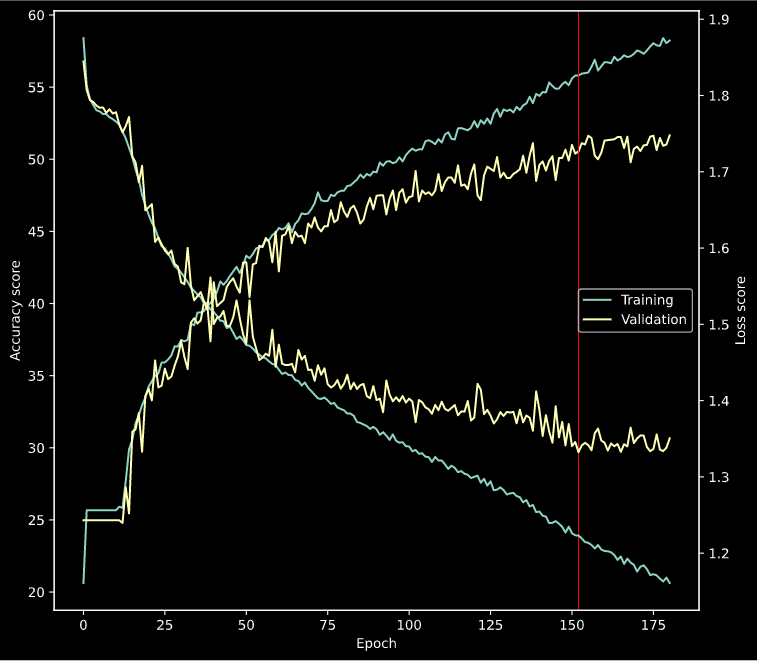
\includegraphics[width=6.75cm]{gambar/eksperimen4b2_grafik1.png}
        \caption{Grafik Performa Per \textit{Epoch} untuk Model E}
        \label{fig:grafikeksperimen4b21}
    \end{subfigure}
    ~~~
    \begin{subfigure}[t]{6.75cm}
        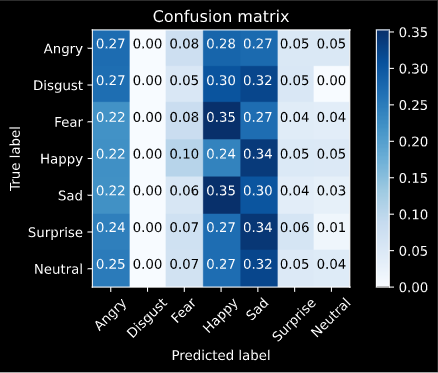
\includegraphics[width=6.75cm]{gambar/eksperimen4b2_matriks1.png}
        \caption{\textit{Confusion Matrix} Performa Model E}
        \label{fig:confusionmatrixeksperimen4b21}
    \end{subfigure}
    ~~~
    \begin{subfigure}[t]{6.75cm}
        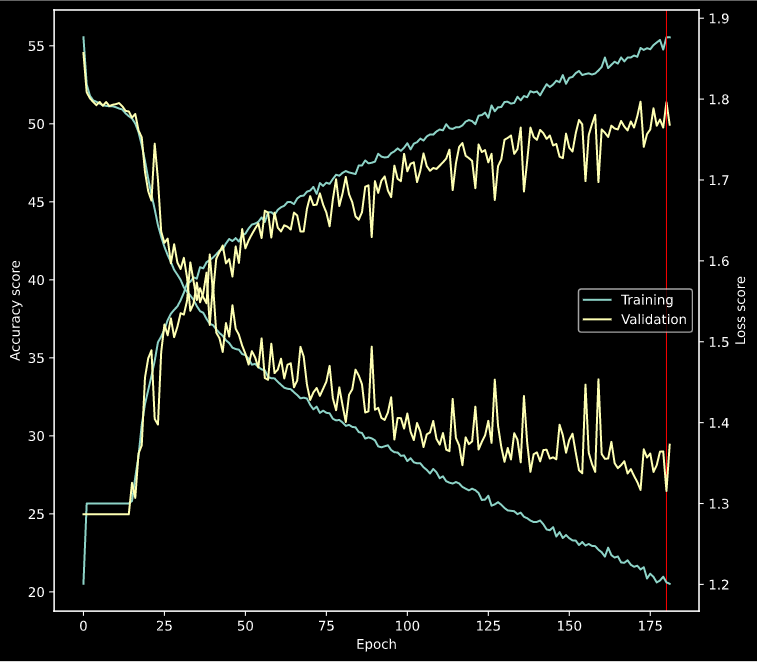
\includegraphics[width=6.75cm]{gambar/eksperimen4b2_grafik2.png}
        \caption{Grafik Performa Per \textit{Epoch} untuk Model N}
        \label{fig:grafikeksperimen4b22}
    \end{subfigure}
    ~~~
    \begin{subfigure}[t]{6.75cm}
        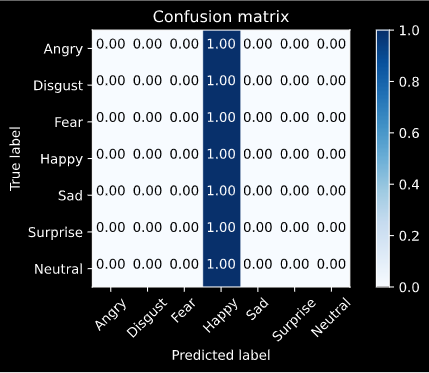
\includegraphics[width=6.75cm]{gambar/eksperimen4b2_matriks2.png}
        \caption{\textit{Confusion Matrix} Performa Model N}
        \label{fig:confusionmatrixeksperimen4b22}
    \end{subfigure}
    \caption{Performa Model \acrshort{gcns} Menggunakan Fitur E + N + M}
    \label{fig:hasileksperimen4b2}
\end{figure}
\begin{figure}[!htb]
    \ContinuedFloat
    \centering
    \begin{subfigure}[t]{6.75cm}
        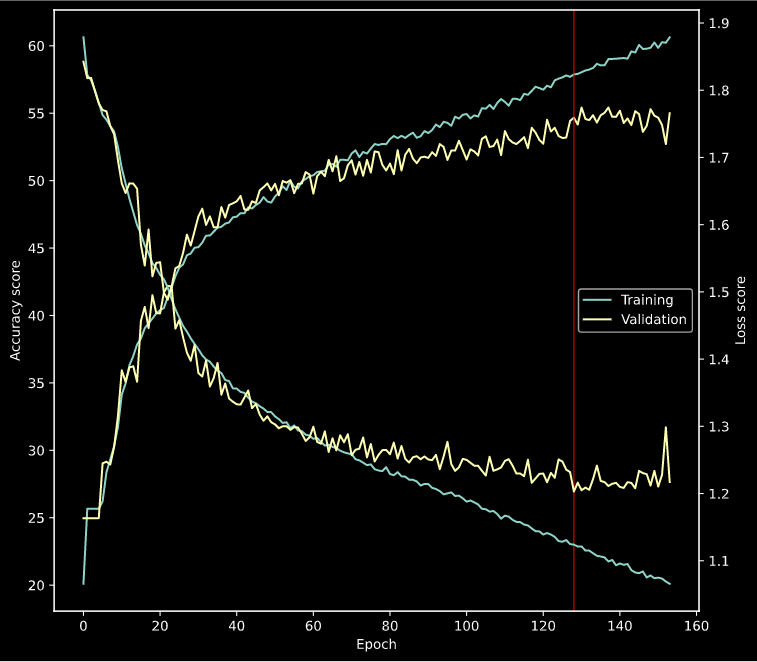
\includegraphics[width=6.75cm]{gambar/eksperimen4b2_grafik3.png}
        \caption{Grafik Performa Per \textit{Epoch} untuk Model M}
        \label{fig:grafikeksperimen4b23}
    \end{subfigure}
    ~~~
    \begin{subfigure}[t]{6.75cm}
        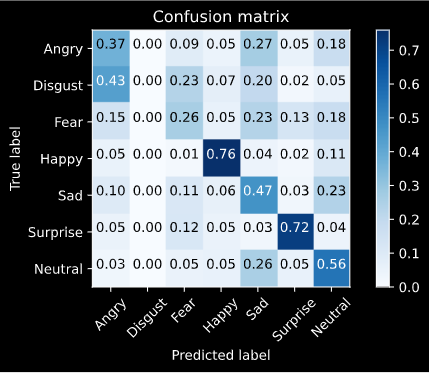
\includegraphics[width=6.75cm]{gambar/eksperimen4b2_matriks3.png}
        \caption{\textit{Confusion Matrix} Performa Model M}
        \label{fig:confusionmatrixeksperimen4b23}
    \end{subfigure}
    ~~~
    \begin{subfigure}[t]{6.75cm}
        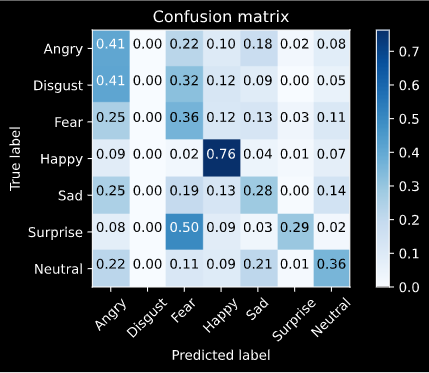
\includegraphics[width=6.75cm]{gambar/eksperimen4b2_matriks4.png}
        \caption{\textit{Confusion Matrix} Performa Model E + N + M Berdasarkan Perhitungan \textit{Simple Average}}
        \label{fig:confusionmatrixeksperimen4b24}
    \end{subfigure}
    ~~~
    \begin{subfigure}[t]{6.75cm}
        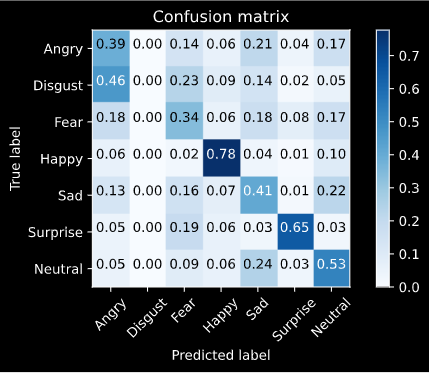
\includegraphics[width=6.75cm]{gambar/eksperimen4b2_matriks5.png}
        \caption{\textit{Confusion Matrix} Performa Model E + N + M Berdasarkan Perhitungan \textit{Weighted Average}}
        \label{fig:confusionmatrixeksperimen4b25}
    \end{subfigure}
    \caption{Performa Model \acrshort{gcns} Menggunakan Fitur E + N + M (Lanjutan)}
\end{figure}
Dalam membandingkan masing-masing dari performa model E, N dan M, terlihat pada Gambar \ref{fig:confusionmatrixeksperimen4b21}--\ref{fig:confusionmatrixeksperimen4b23} bahwa untuk model E dan N memiliki \textit{confusion matrix} yang tidak menarik dan masuk akal. Model E hanya mampu mengenali emosi \textit{angry}, \textit{happy} dan \textit{sad} pada akurasi yang kurang dari 30\%. Sedangkan untuk emosi sisanya tersebar dengan cukup merata pada ketiga label emosi tersebut. Emosi \textit{surprise} dan \textit{neutral} yang umumnya termasuk kelas yang paling mudah untuk dikenali, tidak mampu diprediksi oleh model E. Selanjutnya yang sangat mengejutkan adalah model N hanya mampu mengenali emosi \textit{happy} secara 100\% akurat. Namun, label emosi lainnya juga 100\% gagal diprediksi dan malah dianggap sebagai \textit{happy}. Kemudian untuk model M, performanya dalam mengenali setiap emosi cukup dapat diterima. Sebab memberikan \textit{confusion matrix} yang mirip dengan model \textit{baseline} tanpa augmentasi data.

Di sisi lain, rerata performa model E + N + M memberikan \textit{confusion matrix} yang cukup mirip dengan performa model M. Terutama dalam perhitungan \textit{weighted average}, model memberikan akurasi yang sedikit lebih baik pada pengenalan emosi \textit{angry} dan \textit{fear}. Sedangkan untuk sisanya relatif menurun sedikit.

Dari analisis di atas, diketahui bahwa ketiga fitur wajah tersebut ternyata saling berkaitan satu sama lain pada pengenalan emosi manusia. Namun area bagian mulut memang memberikan kontribusi paling besar dari keseluruhan skenario yang dilakukan. Di sisi lain, rendahnya akurasi model rekognisi emosi untuk tiap-tiap bagian wajah terpisah mengungkapkan bahwa di antara kemungkinan sebabnya adalah adanya perbedaan yang kuat antara orang barat dan timur dalam bagaimana mereka mengekspresikan suatu emosi \shortcite{benitez2017analysis}.

\begin{figure}[t]
    \centering
    \begin{subfigure}[t]{6.75cm}
        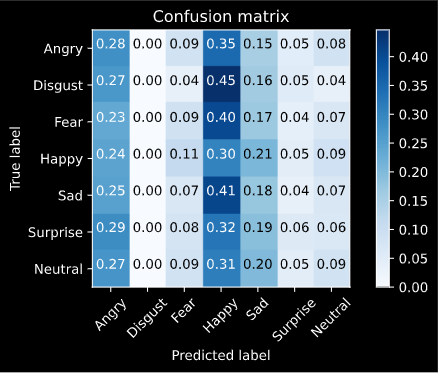
\includegraphics[width=6.75cm]{gambar/eksperimen4b3_matriks1.png}
        \caption{\textit{Confusion Matrix} Performa Model E + N Berdasarkan Perhitungan \textit{Simple Average}}
        \label{fig:confusionmatrixeksperimen4b3}
    \end{subfigure}
    ~~~
    \begin{subfigure}[t]{6.75cm}
        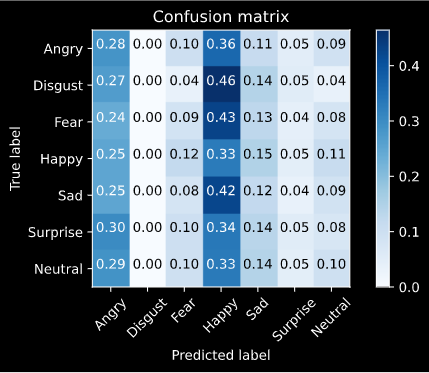
\includegraphics[width=6.75cm]{gambar/eksperimen4b3_matriks2.png}
        \caption{\textit{Confusion Matrix} Performa Model E + N Berdasarkan Perhitungan \textit{Weighted Average}}
        \label{fig:confusionmatrixeksperimen4b3}
    \end{subfigure}
    \caption{Performa Model \acrshort{gcns} Menggunakan Fitur E + N}
    \label{fig:hasileksperimen4b3}
\end{figure}

\begin{figure}[t]
    \centering
    \begin{subfigure}[t]{6.75cm}
        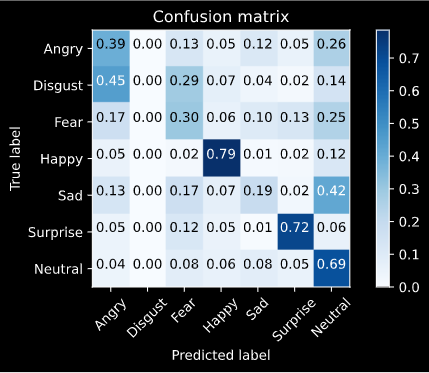
\includegraphics[width=6.75cm]{gambar/eksperimen4b4_matriks1.png}
        \caption{\textit{Confusion Matrix} Performa Model N + M Berdasarkan Perhitungan \textit{Simple Average}}
        \label{fig:confusionmatrixeksperimen4b4}
    \end{subfigure}
    ~~~
    \begin{subfigure}[t]{6.75cm}
        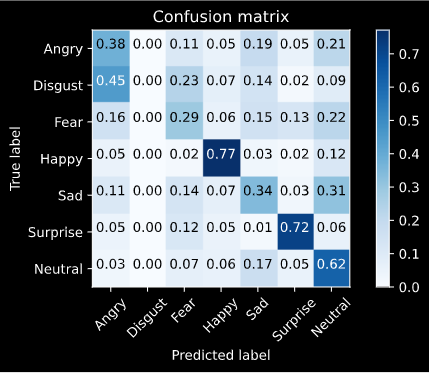
\includegraphics[width=6.75cm]{gambar/eksperimen4b4_matriks2.png}
        \caption{\textit{Confusion Matrix} Performa Model N + M Berdasarkan Perhitungan \textit{Weighted Average}}
        \label{fig:confusionmatrixeksperimen4b4}
    \end{subfigure}
    \caption{Performa Model \acrshort{gcns} Menggunakan Fitur N + M}
    \label{fig:hasileksperimen4b4}
\end{figure}

\begin{figure}[t]
    \centering
    \begin{subfigure}[t]{6.75cm}
        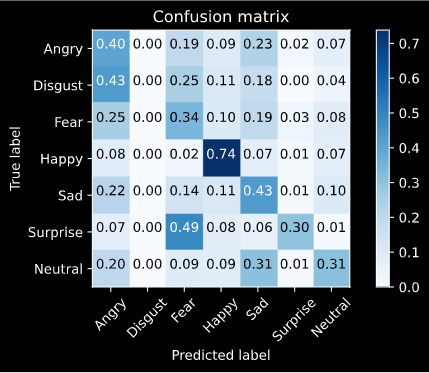
\includegraphics[width=6.75cm]{gambar/eksperimen4b5_matriks1.png}
        \caption{\textit{Confusion Matrix} Performa Model E + M Berdasarkan Perhitungan \textit{Simple Average}}
        \label{fig:confusionmatrixeksperimen4b5}
    \end{subfigure}
    ~~~
    \begin{subfigure}[t]{6.75cm}
        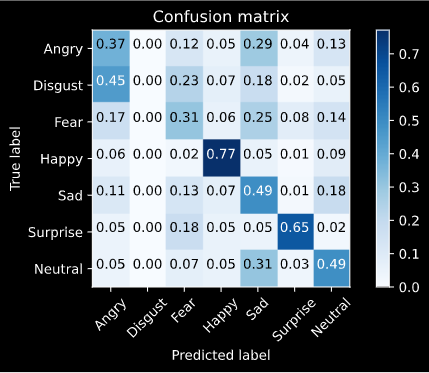
\includegraphics[width=6.75cm]{gambar/eksperimen4b5_matriks2.png}
        \caption{\textit{Confusion Matrix} Performa Model E + M Berdasarkan Perhitungan \textit{Weighted Average}}
        \label{fig:confusionmatrixeksperimen4b5}
    \end{subfigure}
    \caption{Performa Model \acrshort{gcns} Menggunakan Fitur E + M}
    \label{fig:hasileksperimen4b5}
\end{figure}

\begin{figure}[t]
    \centering
    \begin{subfigure}[t]{6.75cm}
        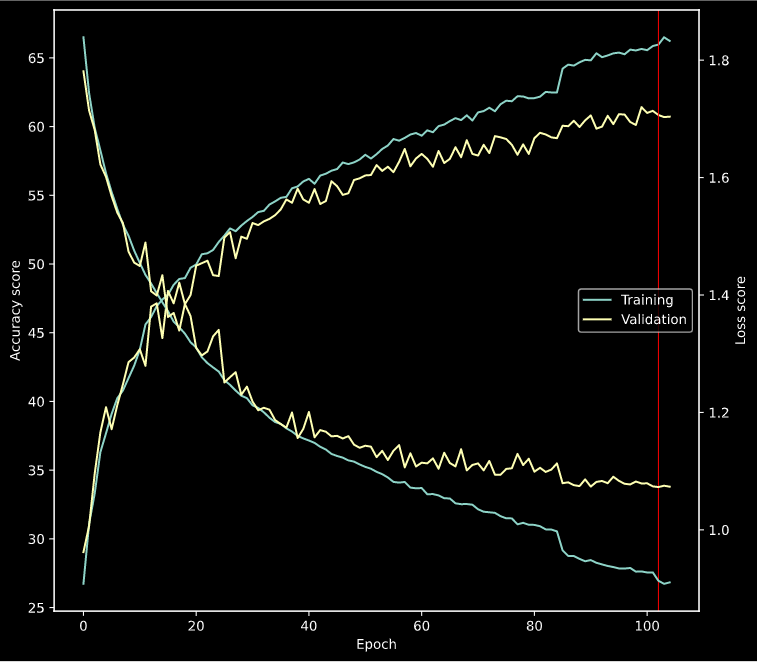
\includegraphics[width=6.75cm]{gambar/eksperimen4b6_grafik1.png}
        \caption{Grafik Performa Per \textit{Epoch} untuk Model EN + NM (\textit{Concat.})}
        \label{fig:confusionmatrixeksperimen4b6}
    \end{subfigure}
    ~~~
    \begin{subfigure}[t]{6.75cm}
        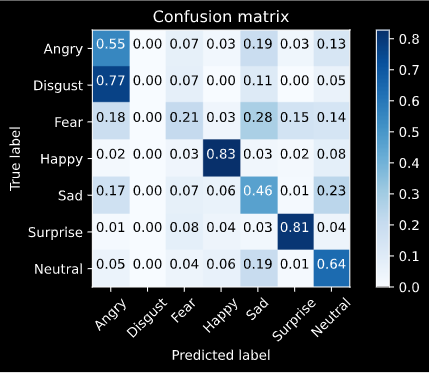
\includegraphics[width=6.75cm]{gambar/eksperimen4b6_matriks1.png}
        \caption{\textit{Confusion Matrix} Performa Model EN + NM (\textit{Concat.})}
        \label{fig:confusionmatrixeksperimen4b6}
    \end{subfigure}
    \caption{Performa Model \acrshort{gcns} Menggunakan Fitur EN + NM (\textit{Concat.})}
    \label{fig:hasileksperimen4b6}
\end{figure}

\begin{figure}[t]
    \centering
    \begin{subfigure}[t]{6.75cm}
        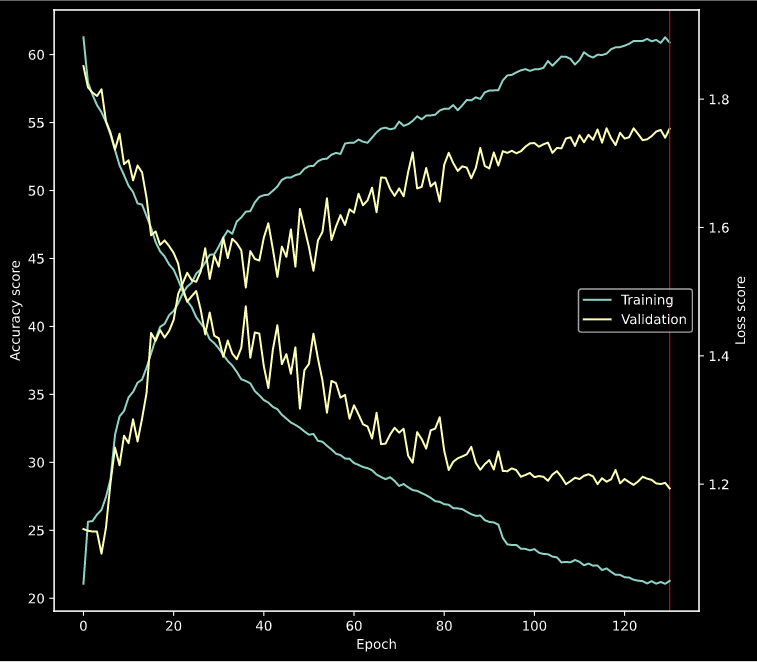
\includegraphics[width=6.75cm]{gambar/eksperimen4b7_grafik1.png}
        \caption{Grafik Performa Per \textit{Epoch} untuk Model E + N + M (\textit{Concat.})}
        \label{fig:confusionmatrixeksperimen4b7}
    \end{subfigure}
    ~~~
    \begin{subfigure}[t]{6.75cm}
        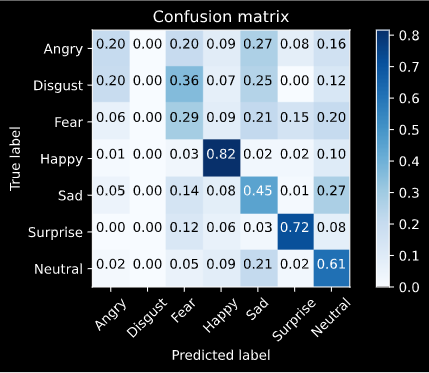
\includegraphics[width=6.75cm]{gambar/eksperimen4b7_matriks1.png}
        \caption{\textit{Confusion Matrix} Performa Model E + N + M (\textit{Concat.})}
        \label{fig:confusionmatrixeksperimen4b7}
    \end{subfigure}
    \caption{Performa Model \acrshort{gcns} Menggunakan Fitur E + N + M (\textit{Concat.})}
    \label{fig:hasileksperimen4b7}
\end{figure}

\begin{figure}[!t]
    \centering
    \begin{subfigure}[t]{6.75cm}
        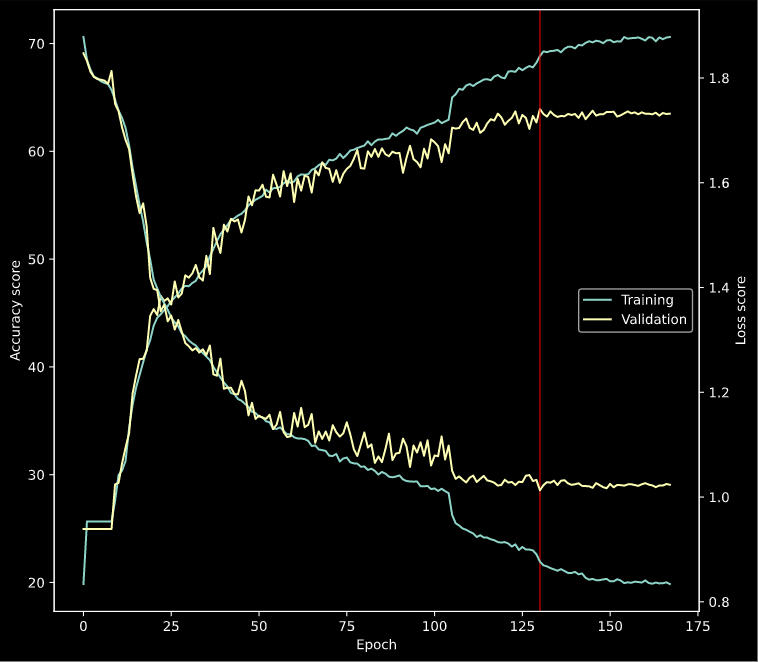
\includegraphics[width=6.75cm]{gambar/eksperimen4b8_grafik1.png}
        \caption{Grafik Performa Per \textit{Epoch} untuk Model ENM}
        \label{fig:confusionmatrixeksperimen4b8}
    \end{subfigure}
    ~~~
    \begin{subfigure}[t]{6.75cm}
        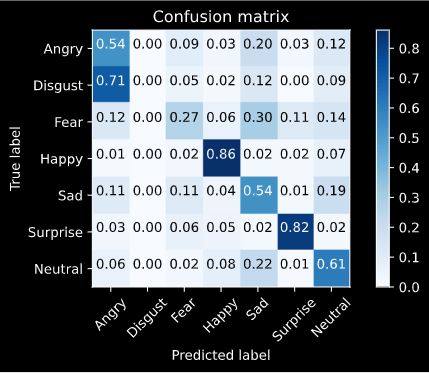
\includegraphics[width=6.75cm]{gambar/eksperimen4b8_matriks1.png}
        \caption{\textit{Confusion Matrix} Performa Model ENM}
        \label{fig:confusionmatrixeksperimen4b8}
    \end{subfigure}
    \caption{Performa Model \acrshort{gcns} Menggunakan Fitur ENM}
    \label{fig:hasileksperimen4b8}
\end{figure}

Meskipun penggunaan fitur bagian mulut memberikan akurasi yang relatif lebih baik daripada yang lain, namun penggabungan dengan fitur lain (area bagian mata dan hidung) malah mengurangi sedikit performa model rekognisi. Di mana model N + M memberikan penurunan yang cukup signifikan pada pengenalan emosi \textit{sad} dengan selisih akurasi 13\%. Akan tetapi untuk emosi \textit{angry}, \textit{fear}, \textit{happy} dan \textit{neutral} meningkat sedikit berturut-turut sebesar 1\%, 3\%, 1\% dan 6\%. Sementara itu, model E + M hanya memberikan peningkatan yang sedikit pada emosi \textit{fear}, \textit{happy} dan \textit{sad} berturut-turut sebesar 5\%, 1\% dan 2\%. Namun mengalami penurunan sebesar 7\% untuk emosi \textit{surprise} dan \textit{neutral}.

Hal ini mungkin terjadi sebagai akibat dari sangat jeleknya akurasi model pada set data bagian mata dan hidung secara terpisah, terutama untuk bagian mata. Sehingga meskipun akurasi model dihitung secara proporsional, performa model menjadi sedikit menurun. Fenomena penurunan performa ini diperkuat oleh perbandingan hasil perhitungan akurasi menggunakan dua teknik yang berbeda, di mana perhitungan \textit{simple average} yang tidak proporsional hampir selalu memberikan nilai akurasi yang lebih rendah dari \textit{weighted average}. Sementara penggabungan fitur bagian mata dan hidung menghasilkan performa yang tidak bisa diterima.

Selanjutnya, model EN + NM yang dilatih menggunakan \textit{network ensemble} pun tidak memiliki keunggulan yang menarik dibandingkan model-model yang sebelumnya. Malahan model E + N + M yang dilatih pada \textit{network ensemble} sangat mengecewakan dalam mengenali emosi \textit{angry}. Namun satu hal yang membedakannya dari semua model sebelumnya adalah kebanyakan data tes berlabel emosi \textit{disgust} dikenali sebagai \textit{fear}. Hal ini membuka sedikit peluang peningkatan performa model dalam mengenali \textit{disgust}, yaitu bahwa sebetulnya tidak benar jika \textit{disgust} ini tidak dapat dibedakan dari \textit{angry}.

Sebagai pertimbangan lain, pada skenario ini dilakukan \textit{training} pada set data hasil \textit{cropping} area wajah penuh, yaitu set data yang disimpan sesaat sebelum masuk ke dalam proses \acrshort{frs}. Sayangnya, teknik \textit{cropping} ini ternyata tidak membuat performa model lebih baik ketimbang tanpa \textit{cropping}. Di sisi lain, tanpa harus mengorbankan performa yang cukup berarti, teknik ini lebih disukai daripada pemodelan menggunakan teknik \acrshort{frs}, sebab membutuhkan waktu \textit{training} yang relatif lebih cepat.

\subsection{Modifikasi Log-\acrshort{gcn} Menjadi \textit{Ensemble} Log-\acrshort{gcns}}
Pada eksperimen ini, penulis mencoba melakukan modifikasi \acrshort{gcn} melalui pengubahan filter Gabor yang dimanfaatkan dalam proses ekstraksi fitur menjadi filter log-Gabor. Namun sebelum mengeksekusi skenario eksperimen terakhir ini, penulis ingin melihat apakah pengubahan filter tersebut dapat memberikan dampak terhadap kinerja model \acrshort{gcn}, sehingga diputuskan bahwa penulis kembali menggunakan set data primer.

Konfigurasi parameter filter log-Gabor yang dipakai pada eksperimen ini dibuat menyerupai konfigurasi filter Gabor terbaik yang sebelumnya. Bedanya, untuk filter log-Gabor, penulis menentukan frekuensi spasial $\text{sf\_0} = 0,0075 / \text{scale}$ sebagai ganti atas variabel \textit{scale} pada filter Gabor. Di mana untuk lapisan konvolusi ke-8 ke bawah menggunakan $\text{scale} = 1,25$, sedangkan sisanya menggunakan $\text{scale} = 1,0$. Perbedaan yang mendasar dari kedua filter ini ditunjukkan pada Gambar \ref{fig:filterloggaborvsgabor}. Di mana bagian daerah dengan frekuensi spasial yang rendah (daerah berwarna hitam) pada filter log-Gabor cenderung cembung mengarah ke dalam. Sedangkan pada filter Gabor, daerah ini cenderung cembung mengarah ke luar.
\begin{figure}[!t]
    \centering
    \begin{subfigure}[t]{14cm}
        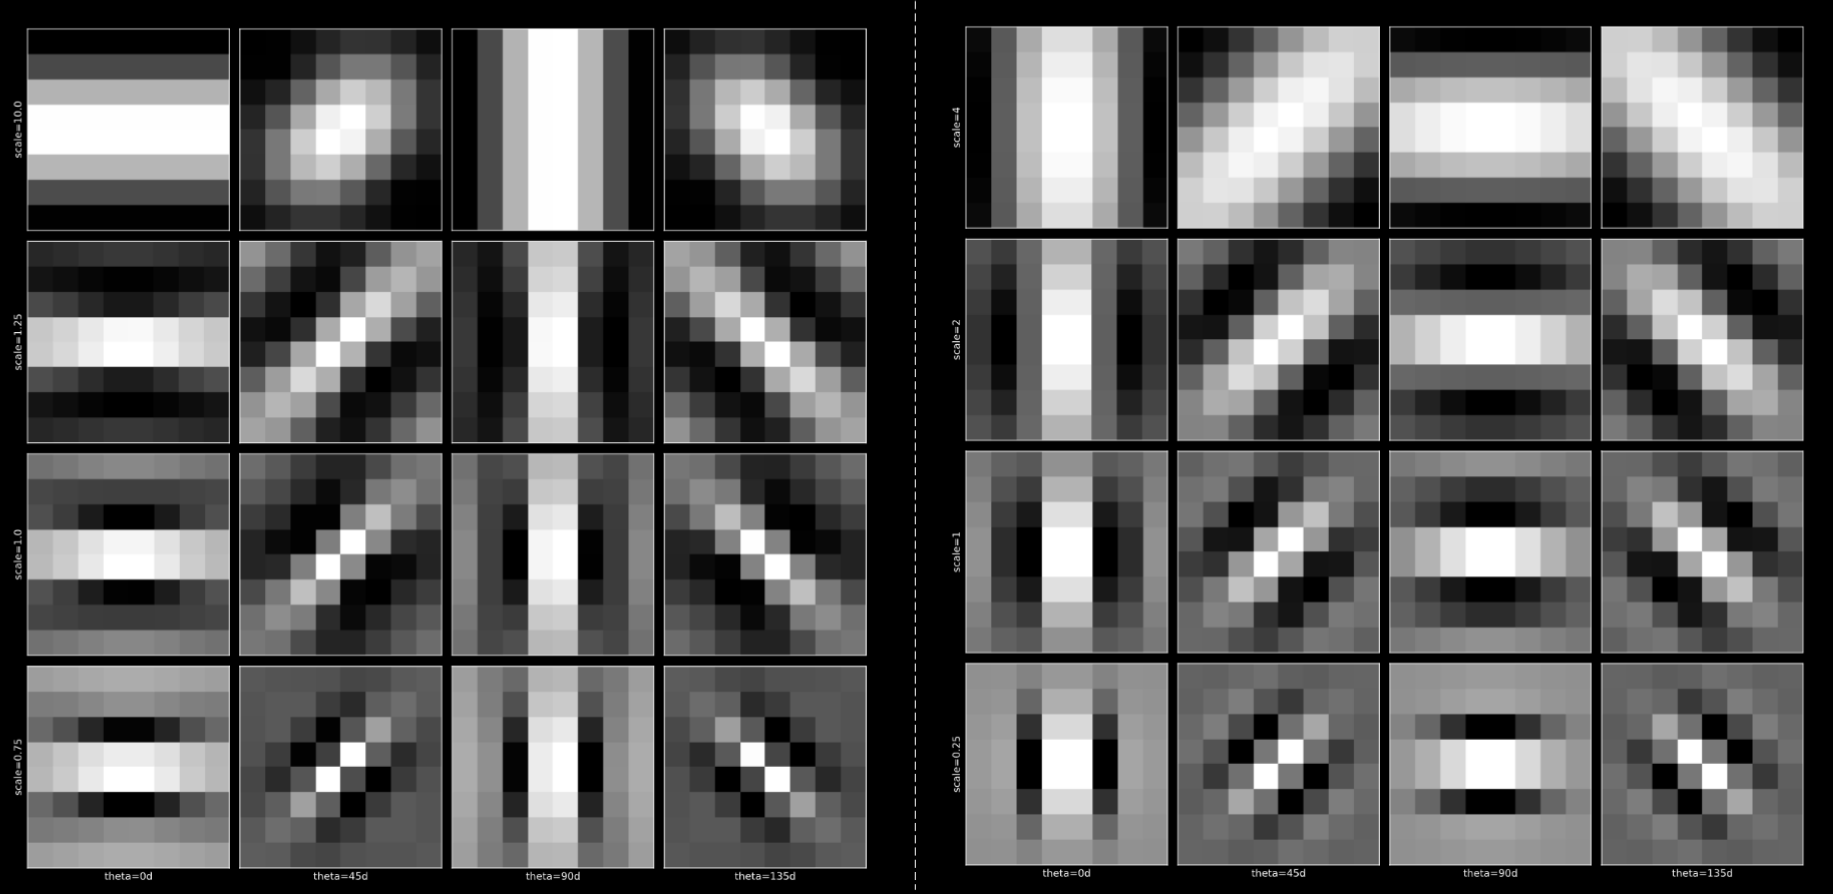
\includegraphics[width=14cm]{gambar/filter_loggaborvsgabor1.png}
        \caption{Filter log-Gabor Versus Gabor pada $8 \times 8$ Piksel}
        \label{fig:filterloggaborvsgabor1}
    \end{subfigure}
    ~~~
    \begin{subfigure}[t]{14cm}
        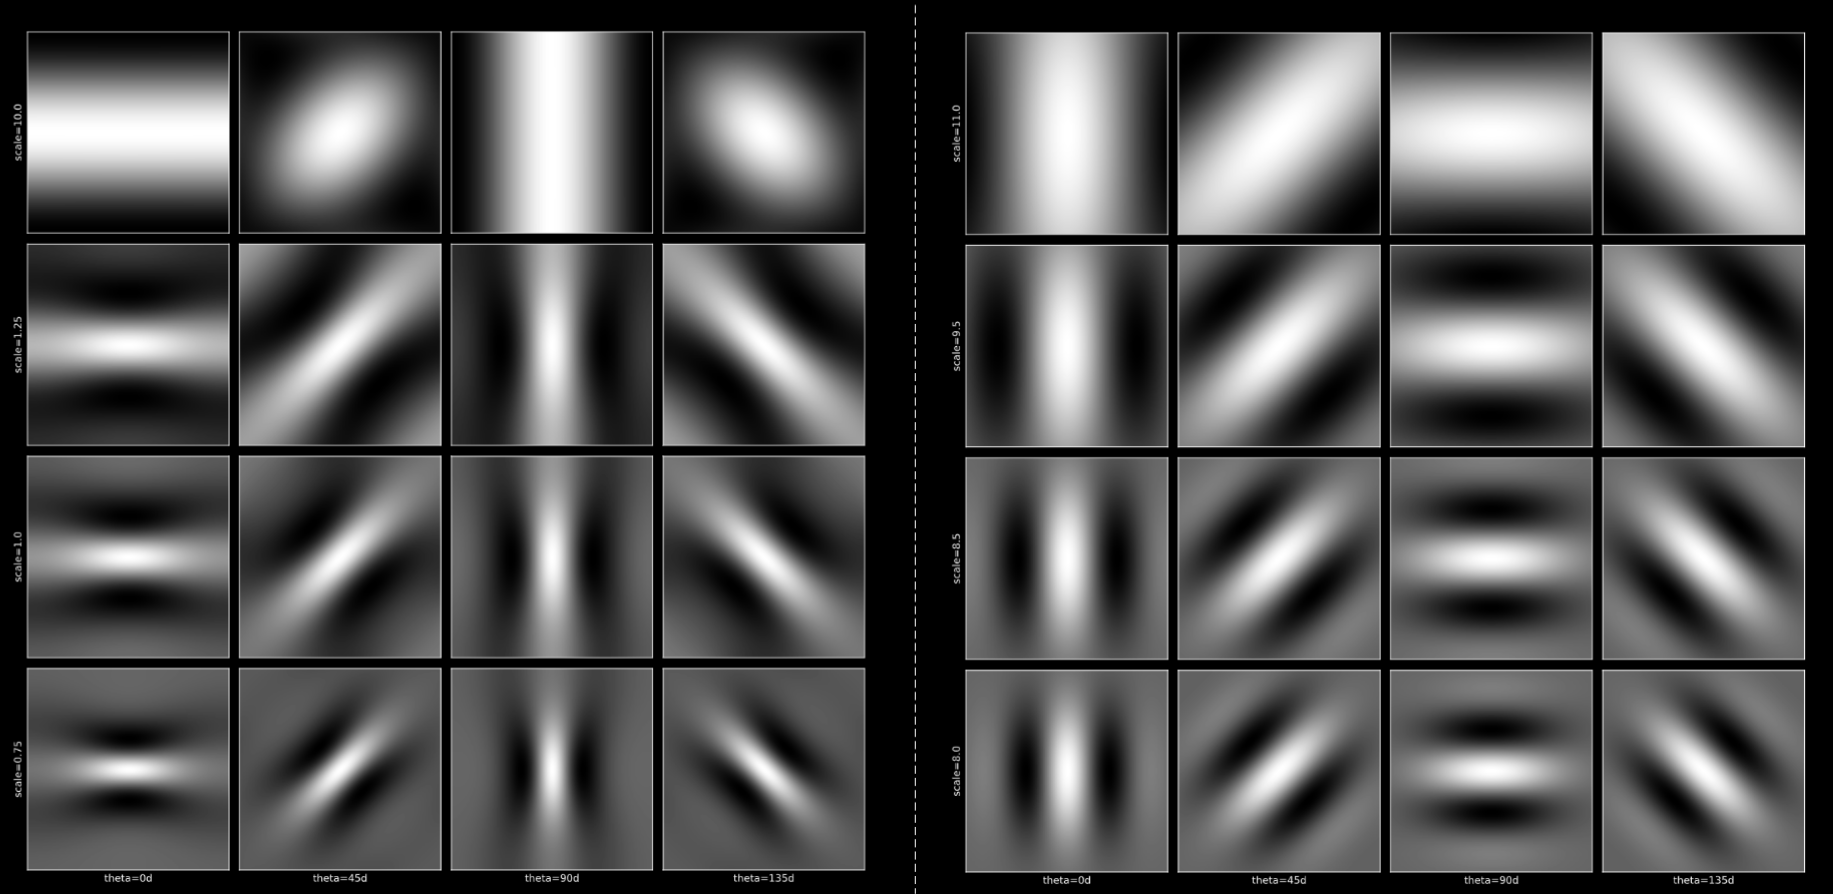
\includegraphics[width=14cm]{gambar/filter_loggaborvsgabor2.png}
        \caption{Filter log-Gabor Versus Gabor pada $100 \times 100$ Piksel}
        \label{fig:filterloggaborvsgabor2}
    \end{subfigure}
    \caption{Beberapa Contoh Perbedaan Filter log-Gabor (Kanan) dan Gabor (Kiri)}
    \label{fig:filterloggaborvsgabor}
\end{figure}

\begin{table}[t]
    \caption{Perbandingan Performa Model \acrshort{gcn} dan Log-\acrshort{gcn}}
    \label{tab:eksperimenloggcn}
    \begin{tabular}{|L{5.4cm}|C{2.6cm}|C{1.5cm}|C{2.7cm}|}
        \hline
        & Akurasi (\%)$^\bigtriangleup$ & \textit{Epoch} & Waktu (jam)$^\bigtriangledown$ \\
        \hline\hline
        Model \acrshort{gcn} & 63,51 & 150 & 7,95 \\
        \hline
        Model Log-\acrshort{gcn} & 65,13 & 155 & 8,38 \\
        \hline
    \end{tabular}
    \footnotesize
    {\raggedright Akurasi---akurasi model pada \textit{testing}; \textit{Epoch}---banyak \textit{epoch} yang dibutuhkan agar model menjadi optimal; Waktu---waktu yang dibutuhkan agar model menjadi optimal; $^\bigtriangleup$Lebih tinggi lebih baik; $^\bigtriangledown$Lebih rendah lebih baik.}
\end{table}
Hasil dari eksperimen pada skenario ini ditampilkan pada Tabel \ref{tab:eksperimenloggcn} di mana terbukti bahwa model log-\acrshort{gcn} memiliki performa yang lebih baik daripada \acrshort{gcn} dengan perbaikan yang cukup jelas pada data berlabel \textit{sad} (Gambar \ref{fig:perbandinganeksperimen3dan5a}). Untuk mendapatkan peningkatan sebesar 1,62\% pada akurasi \textit{testing}, model log-\acrshort{gcn} memerlukan waktu \textit{training} 1,05 kali lebih lama. Model ini menjadi model dengan performa terbaik di atas semua skenario pemodelan pada penelitian ini. Peningkatan akurasi ini bukan akibat dari kebetulan melakukan \emph{training} pada kondisi mesin sedemikian rupa. Sebab berdasarkan dari percobaan tiga kali \emph{training} untuk masing-masing skenario utama pada penelitian ini, biasanya perbedaan akurasi antara model paling buruk dan paling baik berkisar di bawah angka 1,0\%. Kemudian yang amat disayangkan di sini adalah model yang dilatih hingga saat ini masih belum mampu untuk mengenali data berlabel \textit{disgust} dengan benar sama sekali sebagaimana yang ditunjukkan oleh \textit{confusion matrix} pada Gambar \ref{fig:confusionmatrixeksperimen5a}.
\begin{figure}[t]
    \centering
    \begin{subfigure}[t]{6.75cm}
        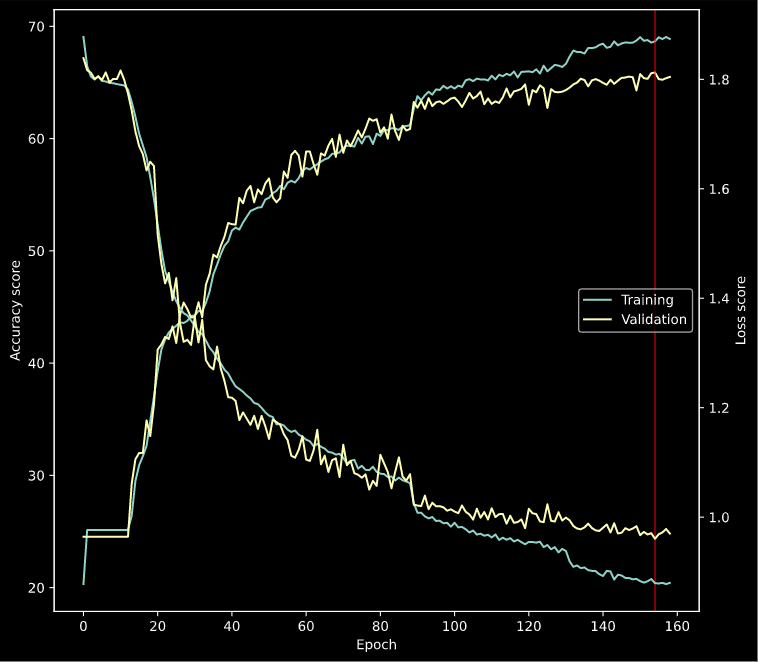
\includegraphics[width=6.75cm]{gambar/eksperimen5a_grafik1.png}
        \caption{Grafik Performa Per \textit{Epoch} untuk Model Log-\acrshort{gcn}}
        \label{fig:confusionmatrixeksperimen5a}
    \end{subfigure}
    ~~~
    \begin{subfigure}[t]{6.75cm}
        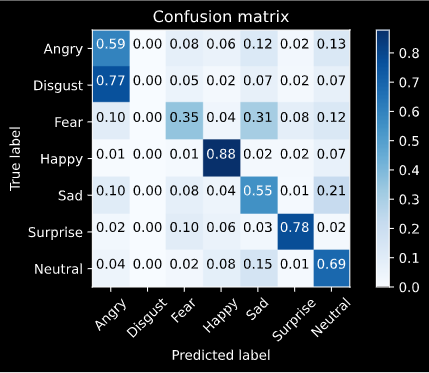
\includegraphics[width=6.75cm]{gambar/eksperimen5a_matriks1.png}
        \caption{\textit{Confusion Matrix} Performa Model Log-\acrshort{gcn}}
        \label{fig:confusionmatrixeksperimen5a}
    \end{subfigure}
    \caption{Performa Model Log-\acrshort{gcn}}
    \label{fig:hasileksperimen5a}
\end{figure}
\begin{figure}[t]
    \centering
    \includegraphics[width=10cm]{gambar/eksperimen3vs5_grafik1.png}
    \caption{Perbandingan Performa Model \acrshort{gcn} dan\\Log-\acrshort{gcn} Per Kelas Emosi}
    \label{fig:perbandinganeksperimen3dan5a}
\end{figure}

Setelah mengetahui bahwa pengubahan filter Gabor menjadi log-Gabor berhasil meningkatkan performa model, penulis melakukan modifikasi log-\acrshort{gcn} menjadi \textit{ensemble} log-\acrshort{gcns}, yaitu pengenaan teknik \acrshort{frs} terhadap arsitektur log-\acrshort{gcn}. Dari berbagai skenario implementasi teknik \acrshort{frs} pada Tabel \ref{tab:eksperimengcnfrs}, penulis mengangkat tiga pendekatan yang menghasilkan kinerja model terbaik untuk dilakukan kembali pada eksperimen tahap ini. Hasilnya diperlihatkan pada Tabel \ref{tab:eksperimenlgcnfrs}.
\begin{table}[t]
    \caption{Perbandingan Performa Berbagai Kombinasi Model \textit{Ensemble} Log-\acrshort{gcns}}
    \label{tab:eksperimenlgcnfrs}
    \begin{tabular}{|C{2.3cm}|C{1cm}|C{1cm}|C{1.2cm}|C{1.8cm}|C{1.8cm}|C{1.8cm}|}
        \hline
        \multicolumn{1}{|c|}{\multirow{3}{*}{Fitur}} & \multicolumn{2}{c|}{\multirow{3}{*}{Waktu (jam)$^\bigtriangledown$}} & \multicolumn{1}{c|}{\multirow{3}{*}{\textit{Epoch}}} & \multicolumn{3}{c|}{Akurasi \textit{Testing} (\%)$^\bigtriangleup$} \\
        \cline{5-7}
        & \multicolumn{2}{c|}{} &  & \multirow{2}{*}{\textit{Single}} & \textit{Simple Average} & \textit{Weighted Average} \\
        \hline\hline
        \multirow{2}{*}{EN + NM} & 3,71 & \multirow{2}{*}{6,91} & 114 & 59,23 & \multirow{2}{*}{64,21} & \multirow{2}{*}{64,21} \\
        \cline{2-2}\cline{4-5}
        & 3,20 &  & 102 & 59,83 &  &  \\
        \hline
        EN + NM (\textit{concat.}) & \multicolumn{2}{c|}{\multirow{2}{*}{8,69}} & \multirow{2}{*}{136} & \multirow{2}{*}{61,27} & \multicolumn{2}{c|}{\multirow{3}{*}{-}} \\
        \cline{1-5}
        ENM & \multicolumn{2}{c|}{4,34} & 86 & 63,07 & \multicolumn{2}{c|}{} \\
        \hline\hline
        EN + NM + ENM & \multicolumn{2}{c|}{\multirow{2}{*}{11,25}} & \multirow{2}{*}{Ibid.} & \multirow{2}{*}{Ibid.} & \multirow{2}{*}{66,25} & \multirow{2}{*}{66,34} \\
        \hline
    \end{tabular}
    \footnotesize
    {\raggedright E---(\textit{Eyes}) area bagian kedua mata; N---(\textit{Nose}) area bagian hidung; M---(\textit{Mouth}) area bagian mulut;\\
    \textit{Epoch}---banyak \textit{epoch} yang dibutuhkan agar model menjadi optimal; Waktu---waktu yang dibutuhkan agar model menjadi optimal; $^\bigtriangleup$Lebih tinggi lebih baik; $^\bigtriangledown$Lebih rendah lebih baik.}
\end{table}

Dari tiga pendekatan \acrshort{frs} ini yang dilakukan pada arsitektur log-\acrshort{gcn}, seluruhnya membutuhkan waktu \textit{training} yang relatif lebih cepat dalam \textit{epoch} yang relatif lebih sedikit dan menghasilkan akurasi pengenalan yang lebih tinggi daripada sebelumnya. Adapun kinerja yang diperoleh oleh tiga pendekatan tersebut memiliki urutan yang sama seperti sebelumnya. Yaitu kinerja terbaik berhasil dicapai oleh model EN + NM yang menggunakan teknik \textit{ensemble} konvensional. Dilanjutkan dengan model EN + NM yang dilatih pada \textit{network ensemble} dan model ENM berturut-turut menempati urutan kedua dan ketiga.

\begin{figure}[t]
    \centering
    \begin{subfigure}[t]{6.75cm}
        \includegraphics[width=6.75cm]{gambar/eksperimen5b1_grafik1.png}
        \caption{Grafik Performa Per \textit{Epoch} untuk Model EN}
        \label{fig:grafikeksperimen5b11}
    \end{subfigure}
    ~~~
    \begin{subfigure}[t]{6.75cm}
        \includegraphics[width=6.75cm]{gambar/eksperimen5b1_matriks1.png}
        \caption{\textit{Confusion Matrix} Performa Model EN}
        \label{fig:confusionmatrixeksperimen5b11}
    \end{subfigure}
    ~~~
    \begin{subfigure}[t]{6.75cm}
        \includegraphics[width=6.75cm]{gambar/eksperimen5b1_grafik2.png}
        \caption{Grafik Performa Per \textit{Epoch} untuk Model NM}
        \label{fig:grafikeksperimen5b12}
    \end{subfigure}
    ~~~
    \begin{subfigure}[t]{6.75cm}
        \includegraphics[width=6.75cm]{gambar/eksperimen5b1_matriks2.png}
        \caption{\textit{Confusion Matrix} Performa Model NM}
        \label{fig:confusionmatrixeksperimen5b12}
    \end{subfigure}
    \caption{Performa Model Log-\acrshort{gcns} Menggunakan Fitur EN + NM}
    \label{fig:hasileksperimen5b1}
\end{figure}
\begin{figure}[t]
    \ContinuedFloat
    \centering
    \begin{subfigure}[t]{6.75cm}
        \includegraphics[width=6.75cm]{gambar/eksperimen5b1_matriks3.png}
        \caption{\textit{Confusion Matrix} Performa Model EN + NM Berdasarkan Perhitungan \textit{Simple Average}}
        \label{fig:confusionmatrixeksperimen5b13}
    \end{subfigure}
    ~~~
    \begin{subfigure}[t]{6.75cm}
        \includegraphics[width=6.75cm]{gambar/eksperimen5b1_matriks4.png}
        \caption{\textit{Confusion Matrix} Performa Model EN + NM Berdasarkan Perhitungan \textit{Weighted Average}}
        \label{fig:confusionmatrixeksperimen5b14}
    \end{subfigure}
    \caption{Performa Model Log-\acrshort{gcns} Menggunakan Fitur EN + NM (Lanjutan)}
\end{figure}
Berdasarkan \textit{confusion matrix} pada Gambar \ref{fig:confusionmatrixeksperimen5b11} dan \ref{fig:confusionmatrixeksperimen5b12}, terlihat bahwa model EN memiliki akurasi yang lebih tinggi pada pengenalan emosi \textit{angry} dengan selisih 14\% dan \textit{sad} dengan selisih 5\%. Ini kembali menekankan bahwa emosi \textit{angry} lebih mudah dikenali menggunakan bagian wajah atas manusia. Adapun model NM relatif cukup lebih baik pada sisanya. Kecuali untuk \textit{disgust}, model EN kembali lebih banyak melakukan kesalahan prediksi sebagai \textit{angry}. Namun kali ini, selisihnya hanya sebesar 2\%. Untuk emosi \textit{fear}, model ini jauh lebih baik dalam pengenalan emosi tersebut dengan kembali lagi model NM memiliki akurasi yang lebih baik ketimbang model EN. Secara umum, sebesar 2,01\% performa \textit{testing}  untuk model EN + NM berhasil ditingkatkan.

Model EN + NM memberikan hasil perhitungan dua teknik rerata berbeda dalam \textit{confusion matrix} yang tepat sama seperti yang tampak pada Gambar \ref{fig:confusionmatrixeksperimen5b13} dan \ref{fig:confusionmatrixeksperimen5b14}. Untuk setiap label emosi, kombinasi kedua model ini mampu memberikan nilai akurasi yang sedikit lebih baik dibandingkan model NM. Namun untuk label \textit{angry}, akurasinya turun sebesar 1\% terhadap model EN. Sementara penyimpangan prediksi emosi \textit{disgust} relatif cukup lebih besar daripada model EN dan NM secara terpisah.

\begin{figure}[!t]
    \centering
    \begin{subfigure}[t]{6.75cm}
        \includegraphics[width=6.75cm]{gambar/eksperimen5b2_grafik1.png}
        \caption{Grafik Performa Per \textit{Epoch} untuk Model EN + NM (\textit{Concat.})}
        \label{fig:grafikeksperimen5b2}
    \end{subfigure}
    ~~~
    \begin{subfigure}[t]{6.75cm}
        \includegraphics[width=6.75cm]{gambar/eksperimen5b2_matriks1.png}
        \caption{\textit{Confusion Matrix} Performa Model EN + NM (\textit{Concat.})}
        \label{fig:confusionmatrixeksperimen5b2}
    \end{subfigure}
    \caption{Performa Model Log-\acrshort{gcns} Menggunakan Fitur EN + NM (\textit{Concat.})}
    \label{fig:hasileksperimen5b2}
\end{figure}
Model EN + NM yang dilatih menggunakan \textit{network ensemble} memiliki akurasi rekognisi yang relatif lebih rendah terhadap model di atas untuk semua kelas emosi kecuali \textit{sad}. Selain dari peningkatan akurasi 2\% untuk emosi \textit{sad}, tidak ditemukan adanya hal-hal yang menarik untuk dibahas baik dari log performa model per \textit{epoch} pada Gambar \ref{fig:grafikeksperimen5b2} maupun dari \textit{confusion matrix} pada Gambar \ref{fig:confusionmatrixeksperimen5b2}. Bahkan jika dibandingkan dengan model EN + NM yang menggunakan \acrshort{gcn} sebelumnya, tidak ada peningkatan yang cukup signifikan. Meskipun secara keseluruhan, akurasinya meningkat sebesar 1,56\%.

\begin{figure}[!t]
    \centering
    \begin{subfigure}[t]{6.75cm}
        \includegraphics[width=6.75cm]{gambar/eksperimen5b3_grafik1.png}
        \caption{Grafik Performa Per \textit{Epoch} untuk Model EN + NM (\textit{Concat.})}
        \label{fig:grafikeksperimen5b3}
    \end{subfigure}
    ~~~
    \begin{subfigure}[t]{6.75cm}
        \includegraphics[width=6.75cm]{gambar/eksperimen5b3_matriks1.png}
        \caption{\textit{Confusion Matrix} Performa Model EN + NM (\textit{Concat.})}
        \label{fig:confusionmatrixeksperimen5b3}
    \end{subfigure}
    \caption{Performa Model Log-\acrshort{gcns} Menggunakan Fitur EN + NM (\textit{Concat.})}
    \label{fig:hasileksperimen5b3}
\end{figure}
Model ENM pada eksperimen ini hanya mendapatkan peningkatan akurasi sebesar 0,99\% terhadap eksperimen sebelumnya. Meskipun demikian, akurasi pengenalan emosi \textit{fear} pada model ini meningkatkan sebesar 8\% sebagaimana yang terlihat dalam \textit{confusion matrix} pada Gambar \ref{fig:confusionmatrixeksperimen5b3}. Performa tersebut dapat diperoleh hanya dalam \textit{epoch} yang relatif jauh lebih sedikit daripada model yang pernah dilatih pada penelitian ini. Dari informasi tersebut, penulis merasa bila masih terdapat peluang untuk meningkatkan akurasi yang diperoleh.

\begin{figure}[!t]
    \ContinuedFloat
    \centering
    \begin{subfigure}[t]{6.75cm}
        \includegraphics[width=6.75cm]{gambar/eksperimen5b4_matriks1.png}
        \caption{\textit{Confusion Matrix} Performa Model EN + NM + ENM Berdasarkan Perhitungan \textit{Simple Average}}
        \label{fig:confusionmatrixeksperimen5b41}
    \end{subfigure}
    ~~~
    \begin{subfigure}[t]{6.75cm}
        \includegraphics[width=6.75cm]{gambar/eksperimen5b4_matriks2.png}
        \caption{\textit{Confusion Matrix} Performa Model EN + NM + ENM Berdasarkan Perhitungan \textit{Weighted Average}}
        \label{fig:confusionmatrixeksperimen5b42}
    \end{subfigure}
    \caption{Performa Model Log-\acrshort{gcns} Menggunakan Fitur EN + NM + ENM}
    \label{fig:hasileksperimen5b4}
\end{figure}
Pada eksperimen ini, penulis juga mencoba melakukan penggabungan terhadap dua pendekatan yang berbeda, yaitu pendekatan holistik dan parsial. Di mana model prediksi ENM dan EN + NM berturut-turut merupakan representasi dari pendekatan holistik dan parsial. Alhasil, model yang dihasilkan mampu mengungguli setiap model yang pernah ada pada penelitian ini dengan peningkatan relatif terbesar pada akurasi pengenalan emosi \textit{fear} dan \textit{neutral}. Sementara itu, kesalahan pengenalan emosi \textit{disgust} sebagai \textit{angry} juga sangat memprihatinkan. Sebagaimana yang tampak melalui \textit{confusion matrix} pada Gambar \ref{fig:confusionmatrixeksperimen5b41} dan \ref{fig:confusionmatrixeksperimen5b42}, perhitungan dua teknik \textit{averaging} tersebut menghasilkan hasil yang hampir serupa. Mungkin sifat ini diturunkan dari sifat model EN + NM itu sendiri. Pencapaian ini membuktikan bahwa pengenalan menggunakan kombinasi data holistik dan parsial lebih akurat ketimbang menggunakan salah satu dari kedua data tersebut. Secara umum, perbandingan performa tiap-tiap model terbaik dari seluruh skenario eksperimen yang dilakukan per kelas emosi ditunjukkan pada Gambar \ref{fig:perbandinganeksperimen1hingga5}.

\begin{figure}[!t]
    \begin{subfigure}{14cm}
        \includegraphics[width=14cm]{gambar/eksperimen1to5_grafik1.png}
        \caption{Perbandingan Performa Tiap-Tiap Model Terbaik Per Kelas Emosi}
    \end{subfigure}

    \begin{subfigure}{14cm}
        \includegraphics[width=14cm]{gambar/eksperimen1to5_grafik2.png}
        \caption{Perbandingan Performa Tiap-Tiap Model Terbaik Secara Keseluruhan}
    \end{subfigure}
    \caption{Perbandingan Performa Tiap-Tiap Model Terbaik dari Seluruh Skenario Eksperimen}
    \label{fig:perbandinganeksperimen1hingga5}
\end{figure}

\section{Evaluasi Akhir}
Analisis secara kuantitatif telah dibahas dengan cukup detail pada bagian-bagian sebelumnya. Oleh karena itu, pada bagian ini akan memaparkan analisis secara kualitatif mengenai peningkatan model terbaik terhadap model \acrshort{cnn} \textit{baseline} yang menggunakan augmentasi data. Penulis berpikir bahwa evaluasi akhir yang terbaik dapat dilakukan melalui penyelidikan kombinasi \textit{facial action unit} per kelas emosi yang berhasil dan tidak berhasil dikenali dengan benar oleh model terbaik secara saksama terhadap beberapa sampel data tes yang diberikan pada Gambar \ref{fig:hasilprediksifalse1}--\ref{fig:hasilprediksitrue6}. Penyelidikan yang dimaksud di sini mengacu kepada \shortciteA{ekman2002facial} dan \shortciteA{zhang2018facial}. Namun, penulis merasa terlalu berlebihan jika evaluasi dilakukan dengan cara demikian. Sebab model terbaik yang berhasil diperoleh secara umum memiliki kinerja yang belum cukup dapat diandalkan, baik diukur secara kuantitatif maupun secara kualitatif.

Pada sistem pengenalan ekspresi wajah di dunia nyata, di mana biasanya kamera diletakkan pada posisi dan sudut yang mampu menjangkau banyak wajah manusia di sebuah tempat kerumunan, set data wajah yang akan diprediksi dalam waktu-waktu tertentu diakuisisi menggunakan teknik deteksi wajah. Sehingga model terbaik yang diusulkan pada penelitian ini lebih cocok diterapkan daripada model \textit{baseline}. Sebab model yang diusulkan dilatih menggunakan set data wajah hasil dari proses deteksi wajah yang serupa. Sementara model \textit{baseline} dilatih menggunakan set data wajah yang juga mengandung selain dari area wajah, sehingga sejumlah informasi yang tidak diperlukan juga ikut terlibat dalam pelatihan model. Dibuktikan dengan pengujian model \textit{baseline} menggunakan set data wajah penuh hanya memberikan nilai akurasi 17,14\% dengan \textit{confusion matrix} yang tertera pada Gambar \ref{fig:hasileksperimen2enm}.
\begin{figure}[t]
    \centering
    \includegraphics[width=6.75cm]{gambar/eksperimen2_matriks2.png}
    \caption{\textit{Confusion Matrix} Performa\\Model \acrshort{cnn} \textit{Baseline} dengan Augmentasi\\Data pada Set Data Wajah Penuh}
    \label{fig:hasileksperimen2enm}
\end{figure}

Selain model yang diusulkan mampu memberikan nilai akurasi yang relatif lebih baik baik pada pengenalan secara umum maupun pada masing-masing kelas emosi kecuali \textit{disgust}, model tersebut juga memberikan nilai \textit{precision} dan \textit{recall} yang secara umum relatif lebih baik ketimbang model \textit{baseline}. Secara berturut-turut, \textit{precision} yang diberikan oleh model \textit{baseline}, yaitu 0,365, 0,359, 0,658, 0,426, 0,801, dan 0,457 untuk emosi \textit{angry}, \textit{fear}, \textit{happy}, \textit{sad}, \textit{surprise} dan \textit{neutral}. Sedangkan \textit{precision} yang diberikan oleh model yang diusulkan secara berturut-turut, yaitu 0,349, 0,446, 0,829, 0,466, 0,850, dan 0,579. Adapun \textit{precision} untuk emosi \textit{disgust} tidak bisa dihitung karena memberikan perhitungan yang tidak terdefinisi. Jelas terlihat bahwa selain untuk emosi \textit{angry}, \textit{precision} yang diberikan oleh model yang diusulkan relatif lebih baik ketimbang model \textit{baseline}. Penurunan nilai \textit{precision} yang diberikan oleh model yang diusulkan terhadap model \textit{baseline} pada prediksi emosi \textit{angry} terjadi akibat meningkatnya kesalahan prediksi emosi \textit{disgust} menjadi \textit{angry}. Jika tanpa melibatkan kelas \textit{disgust}, perhitungan rata-rata dari \textit{precision} untuk model \textit{baseline} dan model yang diusulkan secara berturut-turut menghasilkan 0,511 dan 0,586.

Model yang diusulkan membutuhkan sumber daya komputasi yang relatif lebih besar, baik ketika \textit{training} maupun prediksi, ketimbang model \textit{baseline}. Di luar dari waktu \textit{training} yang lama sebagaimana yang telah dipaparkan sebelumnya, performa kedua model tersebut dalam memprediksi set data tes FER-2013 berjumlah 3.331 data gambar wajah menggunakan spesifikasi komputer dan sistem yang telah disebutkan dalam penelitian ini tertera pada Tabel \ref{tab:perbandinganperformates}. Tampak bahwa model yang diusulkan memerlukan konsumsi memori yang lebih boros tiga kali lipat dan waktu prediksi yang lebih lama sepuluh kali lipat. Data tabel tersebut tidak bisa dijadikan sebagai acuan dalam estimasi perhitungan kecepatan prediksi dalam \textit{frame per second} (FPS) ketika produksi, di mana berbagai macam faktor terlibat seperti ukuran gambar input, kecepatan algoritma \textit{face detection}, kecepatan algoritma \acrshort{frs} dan lain-lain.
\begin{table}[t]
    \caption{Perbandingan Performa Prediksi Model \acrshort{cnn} \textit{Baseline} dan Log-\acrshort{gcn}\\(EN + NM + ENM) pada Set Data Tes FER-2013}
    \label{tab:perbandinganperformates}
    \begin{tabular}{|L{7.1cm}|C{2.8cm}|C{2.8cm}|}
        \hline
        & Memori (MiB) & Waktu (sekon) \\
        \hline\hline
        Model \acrshort{cnn} \textit{Baseline} & 577 & 1,55 \\
        \hline
        Model Log-\acrshort{gcn} (EN + NM + ENM) & 1.523 & 15,98 \\
        \hline
    \end{tabular}
    \footnotesize
    {\raggedright Waktu yang diukur adalah waktu prediksi seluruh data tes FER-2013 menggunakan spesifikasi komputer dan sistem dalam penelitian ini.}
\end{table}

Emosi berlabel \textit{disgust} tidak mampu sama sekali dikenali dengan benar baik oleh model \textit{baseline} maupun oleh model yang diusulkan. Bahkan model yang diusulkan lebih banyak salah memprediksi emosi tersebut sebagai \textit{angry}. Meskipun kesalahan prediksi ini telah menghancurkan angka presisi dalam pengenalan emosi \textit{angry}, penulis tidak melihat signifikansi dalam hal ini yang mengakibatkan menurunnya performa model secara umum dalam memprediksi setiap emosi terutama \textit{angry} dan \textit{disgust} dengan benar. Terlebih lagi, kesalahan prediksi data berlabel \textit{disgust} menjadi \textit{angry} masih mendapatkan toleransi. \shortciteA{widen2013children} menyimpulkan bahwa mayoritas anak-anak pada usia delapan tahun menyatakan bahwa ekspresi wajah \textit{disgust} mengindikasikan emosi \textit{angry}. Dan hanya setengah dari anak-anak berumur sekitar sembilan tahun yang menganggap bahwa ekspresi wajah \textit{disgust} mengindikasikan emosi \textit{disgust}. Bahkan sebagian dari orang-orang dewasa pun salah mengartikan ekspresi wajah \textit{disgust} sebagai \textit{angry} \shortcite{widen2010disgust}. Setengah dari mereka justru memasukkan ekspresi wajah \textit{disgust} sebagai emosi \textit{angry} dan seperempat dari mereka memasukkan \textit{angry} sebagai \textit{disgust} \shortcite{widen2004anger}. Hal ini membuktikan bahwa sebenarnya orang-orang mempertanyakan mengenai perbedaan emosi \textit{disgust} dan \textit{angry} itu sendiri. Bagaimana pun juga, kedua emosi tersebut sama-sama tergolong ke dalam kelompok emosi negatif. Menurut orang-orang yang memiliki kecemasan sosial, emosi \textit{disgust} dinilai lebih negatif daripada \textit{angry} \shortcite{amir2010disgust}.

Secara umum, akurasi model yang diusulkan dapat mengungguli akurasi model \textit{baseline} seperti yang telah dibahas sebelumnya. Dengan akurasi yang diperoleh tersebut, model yang diusulkan berhasil mencapai \textit{human accuracy} pada set data FER-2013, yaitu 65$\pm$5\% \shortcite{goodfellow2013challenges}. Namun, jika ditinjau dari kemampuan rekognisi per label emosi, model hanya mendapatkan \textit{human accuracy} untuk label \textit{angry}, \textit{happy}, \textit{surprise} dan \textit{neutral}.

% Akhirnya, evaluasi dilakukan terhadap model terbaik yang berhasil dibangun hingga saat ini. Evaluasi dilakukan melalui penyelidikan secara saksama pada beberapa sampel data tes baik yang berhasil maupun yang gagal diprediksi dengan benar. Berdasarkan sejumlah sampel data tes berlabel emosi yang berhasil dikenali dengan benar pada Gambar \ref{fig:hasilprediksitrue1}--\ref{fig:hasilprediksitrue6}, model berhasil mengenali tiap-tiap emosi tersebut pada kombinasi tanda-tanda pada raut wajah yang dijabarkan pada Tabel \ref{tab:indikatorekspresiwajah}.
% \begin{table}[t]
%     \caption{Beberapa Kombinasi Sinyal pada Raut Wajah per Emosi yang Berhasil Dikenali oleh Model Terbaik}
%     \label{tab:indikatorekspresiwajah}
%     \small
%     \begin{tabular}{|C{1.5cm}|L{8.15cm}|L{3cm}|}
%         \hline
%         Label & \multicolumn{1}{C{8.15cm}|}{Kombinasi Sinyal$^\odot$} & \multicolumn{1}{C{3cm}|}{Sampel Gambar$^\oplus$} \\
%         \hline\hline
%         \textit{Angry} & Mata menyipit, mulut sedikit terbuka dengan gigi terkatup dan alis bagian dalam sedikit turun & B1K1, B2K5, B3K1, B4K10, B5K1 \\
%         \cline{2-3}
%         & Mata menyipit, kepala sedikit tertunduk (atau kepala miring ke samping), mata melihat ke depan, mulut terkatup rapat dan alis bagian dalam sedikit turun & B1K7, B1K10, B2K6, B2K7, B3K10 \\
%         \cline{2-3}
%         & Mata menyipit, mulut terbuka lebar dan alis dalam sedikit turun & B1K4, B1K5, B2K1, B2K4, B3K4 \\
%         \cline{2-3}
%         & Mata melotot, mulut terbuka separuh dan dagu condong ke depan & \multirow{2}{*}{B3K6} \\
%         \cline{2-3}
%         & Mata melirik ke samping dan mulut terkatup & B4K3 \\
%         \hline
%         \textit{Fear} & Mulut terkatup dengan jari-jari tangan menutupi mulut (atau jari-jari tangan tergigit) dan mata terbuka normal hingga melotot & B4K3, B1K9, B2K1, B2K5, B3K4, B5K8 \\
%         \cline{2-3}
%         & Mata menyipit dan pipi hingga pelipis tertutup jari-jari tangan & B1K1, B1K2, B3K2, B3K9, B4K2 \\
%         \hline
%         \textit{Happy} & Bibir bagian luar naik (melengkung ke bawah), mulut terbuka sedikit (terkadang menunjukkan gigi) dan mata terbuka normal & \multirow{3}{3cm}{Rata-rata} \\
%         \hline
%         \textit{Sad} & Salah satu sisi wajah tertutup jari-jari tangan, bibir bagian luar turun sedikit dan mata melirik ke bawah/samping & B3K3, B3K5, B4K7, B4K8, B5K2 \\
%         \cline{2-3}
%         & Salah satu sisi wajah tertutup jari-jari tangan, bibir bagian luar turun sedikit dan mata melirik ke bawah/samping & B3K3, B3K5, B4K7, B4K8, B5K2 \\
%         \cline{2-3}
%         & Mata terbuka normal hingga melotot, bibir bawah terlipat ke dalam/luar dan mulut terbuka sedikit/separuh & B1K3, B1K9, B2K3, B3K4, B3K6 \\
%         \cline{2-3}
%         & Mata menyipit, alis bagian dalam naik dan mulut terkatup rapat & B1K6, B2K2, B2K6, B4K1, B5K2 \\
%         \hline
%         \textit{Surprise} & Mata melotot dan mulut terbuka lebar & Rata-rata \\
%         \cline{2-3}
%         & Mata melotot, mulut terbuka separuh hingga lebar dan jari-jari tangan menyentuh pipi (atau menutupi mulut) & B1K1, B1K3, B1K6, B3K6, B3K8 \\
%         \hline
%     \end{tabular}
%     \footnotesize
%     {\raggedright $^\odot$Tanda diukur relatif terhadap ekspresi wajah normal; $^\oplus$BbKk---Baris ke-b Kolom ke-k pada matriks gambar yang sesuai}
% \end{table}

% Fenomena perubahan kecil pada ekspresi wajah seseorang yang seperti ini umumnya disebut sebagai \textit{micro-expression} \shortcite{zhang2020cross}.

\begin{figure}[t]
    \centering
    \includegraphics[width=14cm]{gambar/contoh_hasil_prediksi_false_angry.png}
    \caption{Beberapa Contoh Kesalahan Prediksi Emosi \textit{Angry} oleh Model Terbaik (Label Prediksi $|$ Label Sebenarnya)}
    \label{fig:hasilprediksifalse1}
\end{figure}

\begin{figure}[t]
    \centering
    \includegraphics[width=14cm]{gambar/contoh_hasil_prediksi_false_fear.png}
    \caption{Beberapa Contoh Kesalahan Prediksi Emosi \textit{Fear} oleh Model Terbaik (Label Prediksi $|$ Label Sebenarnya)}
    \label{fig:hasilprediksifalse2}
\end{figure}

\begin{figure}[t]
    \centering
    \includegraphics[width=14cm]{gambar/contoh_hasil_prediksi_false_happy.png}
    \caption{Beberapa Contoh Kesalahan Prediksi Emosi \textit{Happy} oleh Model Terbaik (Label Prediksi $|$ Label Sebenarnya)}
    \label{fig:hasilprediksifalse3}
\end{figure}

\begin{figure}[t]
    \centering
    \includegraphics[width=14cm]{gambar/contoh_hasil_prediksi_false_sad.png}
    \caption{Beberapa Contoh Kesalahan Prediksi Emosi \textit{Sad} oleh Model Terbaik (Label Prediksi $|$ Label Sebenarnya)}
    \label{fig:hasilprediksifalse4}
\end{figure}

\begin{figure}[t]
    \centering
    \includegraphics[width=14cm]{gambar/contoh_hasil_prediksi_false_surprise.png}
    \caption{Beberapa Contoh Kesalahan Prediksi Emosi \textit{Surprise} oleh Model Terbaik (Label Prediksi $|$ Label Sebenarnya)}
    \label{fig:hasilprediksifalse5}
\end{figure}

\begin{figure}[t]
    \centering
    \includegraphics[width=14cm]{gambar/contoh_hasil_prediksi_false_neutral.png}
    \caption{Beberapa Contoh Kesalahan Prediksi Emosi \textit{Neutral} oleh Model Terbaik (Label Prediksi $|$ Label Sebenarnya)}
    \label{fig:hasilprediksifalse6}
\end{figure}

\begin{figure}[!t]
    \centering
    \includegraphics[width=14cm]{gambar/contoh_hasil_prediksi_true_angry.png}
    \caption{Beberapa Contoh Keberhasilan Prediksi Emosi \textit{Angry} oleh Model Terbaik}
    \label{fig:hasilprediksitrue1}
\end{figure}

\begin{figure}[!t]
    \centering
    \includegraphics[width=14cm]{gambar/contoh_hasil_prediksi_true_fear.png}
    \caption{Beberapa Contoh Keberhasilan Prediksi Emosi \textit{Fear} oleh Model Terbaik}
    \label{fig:hasilprediksitrue2}
\end{figure}

\begin{figure}[!t]
    \centering
    \includegraphics[width=14cm]{gambar/contoh_hasil_prediksi_true_happy.png}
    \caption{Beberapa Contoh Keberhasilan Prediksi Emosi \textit{Happy} oleh Model Terbaik}
    \label{fig:hasilprediksitrue3}
\end{figure}

\begin{figure}[!t]
    \centering
    \includegraphics[width=14cm]{gambar/contoh_hasil_prediksi_true_sad.png}
    \caption{Beberapa Contoh Keberhasilan Prediksi Emosi \textit{Sad} oleh Model Terbaik}
    \label{fig:hasilprediksitrue4}
\end{figure}

\begin{figure}[!t]
    \centering
    \includegraphics[width=14cm]{gambar/contoh_hasil_prediksi_true_surprise.png}
    \caption{Beberapa Contoh Keberhasilan Prediksi Emosi \textit{Surprise} oleh Model Terbaik}
    \label{fig:hasilprediksitrue5}
\end{figure}

\begin{figure}[!t]
    \centering
    \includegraphics[width=14cm]{gambar/contoh_hasil_prediksi_true_neutral.png}
    \caption{Beberapa Contoh Keberhasilan Prediksi Emosi \textit{Neutral} oleh Model Terbaik}
    \label{fig:hasilprediksitrue6}
\end{figure}

% https://www.youtube.com/results?search_query=video+pembelajaran+di+kelas, https://www.youtube.com/watch?v=qKCl8Yw4-H4, https://www.youtube.com/watch?v=fOuuTL_dATI

% Meskipun pelabelannya dilakukan oleh manusia, namun sayangnya masih belum cukup akurat. Maka dari itu, FER+ \shortcite{barsoum2016training} dibuat melalui penandaan ulang set data FER-2013 oleh sepuluh orang pengamat sehingga menghasilkan akurasi yang lebih baik \shortcite{georgescu2019local}. FER+ tersedia dengan lisensi MIT secara publik di https://github.com/Microsoft/FERPlus.
